\section{ECP ST Planning, Execution, Tracking and Assessment}\label{sect:PETA}
During the last 2 years, the ECP ST has introduced the E4S and SDKs.  New approaches have been established for project planning, execution, tracking, and assessment by using a tailored earned value management system that enables iterative and incremental refinement to its planning process.  The team has also revised its key performance parameter (KPP) to be solely focused on measuring capability integration into client environments.  An assessment process was developed and used that has led to significant changes in the number and scope of L4 subprojects.

\subsection{ECP ST Architecture and Design}
The ECP is taking an approach of co-design across all its principal technical areas: Application Development (AD), ST, and Hardware and Integration (HI). For the ECP ST, this means that its requirements are based on input from other areas, and there is a tight integration of the software products within the software stack and with applications and the evolving hardware. 

The ECP ST portfolio of projects is intended to address the aforementioned exascale challenges and requirements. The ECP is not developing the entire software stack for an exascale system. For example, vendors are expected to provide the core software that comes with the system---in many cases, by leveraging ECP and other open-source efforts. Examples of vendor-provided software include operating systems; file systems; compilers for C, C++, Fortran, and so on, increasingly derived from the LLVM community ecosystem to which the ECP contributes; basic math libraries; system monitoring tools; schedulers; debuggers; vendor performance tools; MPI based on ECP-funded projects; OpenMP with features from ECP-funded projects; and data-centric stack components. The ECP develops other, mostly higher level software that is needed by applications and is not vendor specific. ECP-funded software activities are concerned with extreme scalability, exposing additional parallelism, unique requirements of exascale hardware, and performance-critical components. Other software that aids in developer productivity is needed and could come from third-party, open-source efforts.

The ST portfolio includes both ASCR and NNSA ATDM-funded efforts. The memorandum of understanding established between DOE SC and NNSA has formalized this effort.  Whenever possible, ASCR and ATDM efforts are treated uniformly in ECP ST planning and assessment activities.

ST also plans to increase integration within the ST portfolio through the increased use of software components and application composition vs. monolithic application design. One important transition that ECP can accelerate is the increased development and delivery of reusable scientific software components and libraries. Although math and scientific libraries have long been a successful element of the scientific software community, their use can be expanded to include other algorithms and software capabilities so that applications can be considered more of an aggregate composition of reusable components than a monolithic code that uses libraries tangentially.

To accelerate this transition, a greater commitment on the part of software component developers is needed to provide reliable and portable software that users can consider to be part of the software ecosystem in much the same way users depend on MPI and compilers. However, application developers must be expected to participate as clients and users of reusable components, using capabilities from components, transitioning away from---or keeping a backup option of---their own custom capabilities.

\subsubsection{The Extreme-Scale Scientific Software Stack}\label{subsubsect:e4s}
In October 2020, the ECP ST released V1.2 of the E4S.\footnote{\url{http://e4s.io}} E4S contains a collection of the software products to which ECP ST contributes.  E4S is the primary conduit for providing easy access to ECP ST capabilities for the ECP and the broader community.  E4S is also the ECP ST vehicle for regression and integration testing across DOE pre-exascale and exascale systems.

\begin{figure}
		\centering
		\fbox{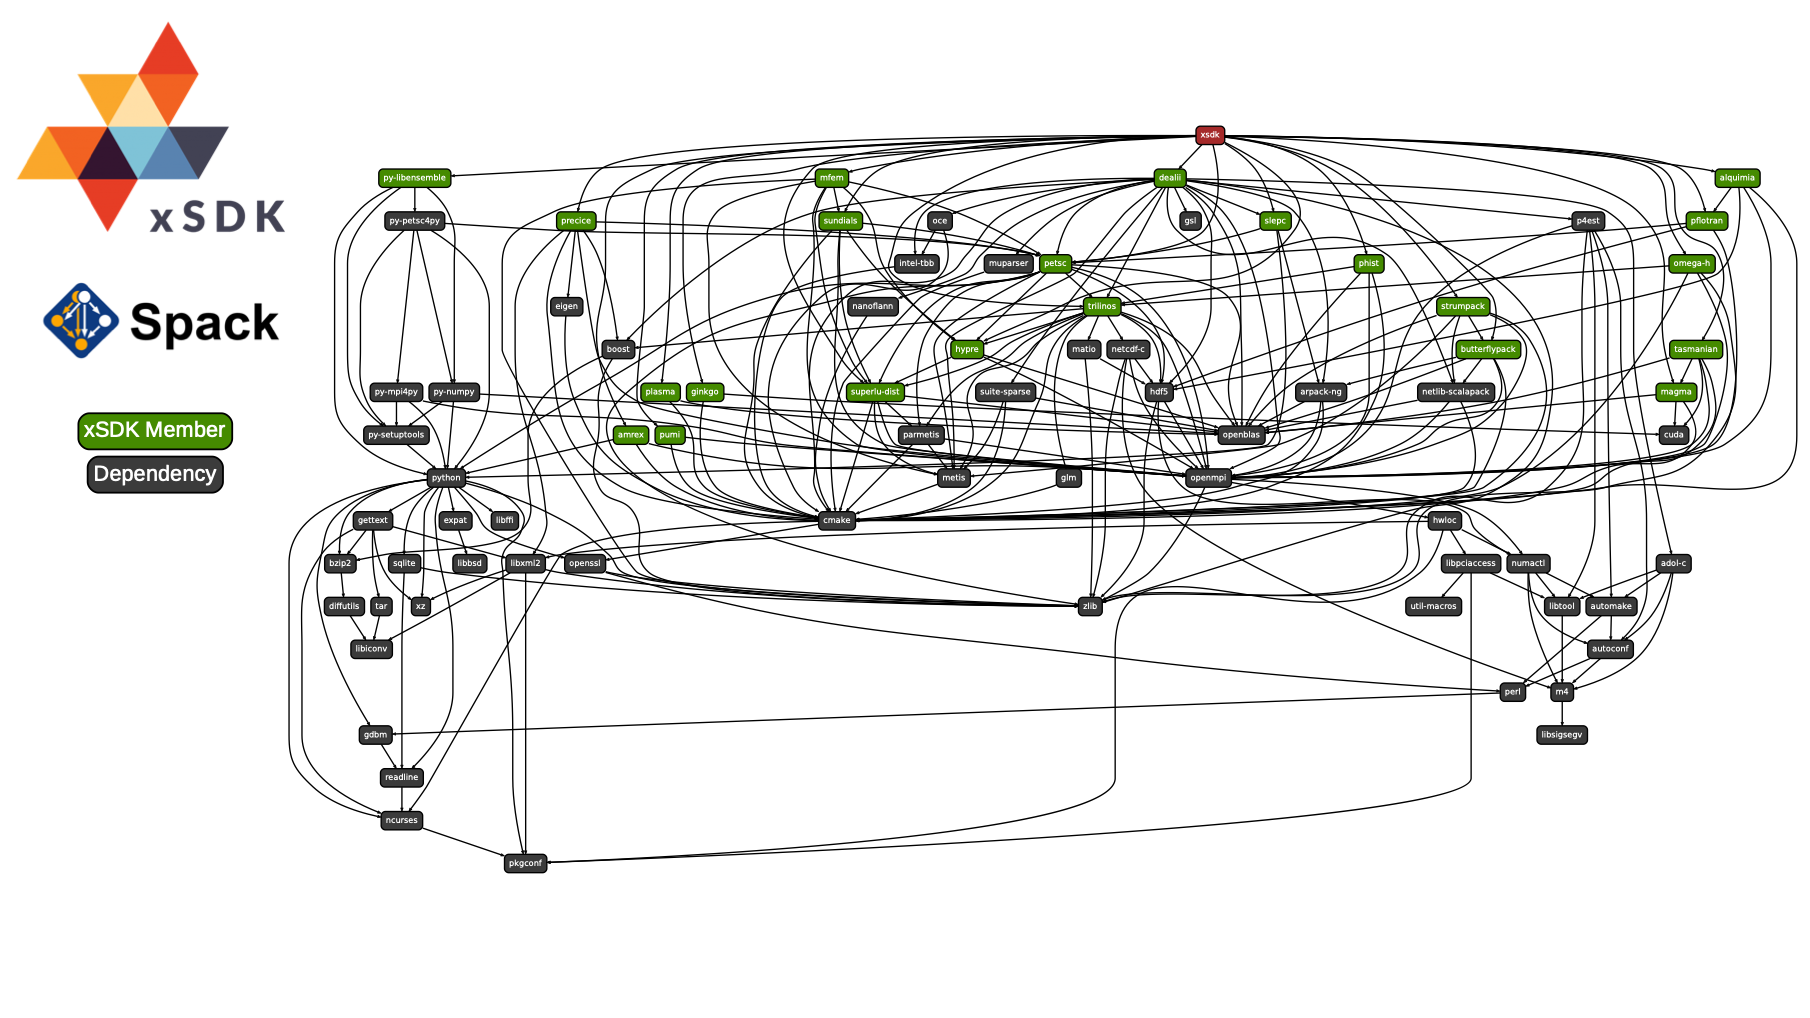
\includegraphics[width=0.9\linewidth]{E4S-Build-Tree}}
	\caption{Using Spack~\cite{gamblin+:ecp18-spack-tutorial}, E4S builds a comprehensive software stack.  As ECP ST efforts proceed, E4S will be used for continuous integration testing, providing developers with rapid feedback on regression errors and providing user facilities with a stable software base as the team prepares for exascale platforms.  This diagram shows how E4S builds ECP products via an SDK target, which are the math libraries' SDK, called xSDK in this example.  The SDK target then builds all products that are part of the SDK (see Figure~\ref{fig:sdk-definition1-0} for SDK groupings), first defining and building external software products. Green-labeled products are part of the SDK. The blue label indicates expected system tools, which, in this case, is a particular version of Python.  Black-labeled products are expected to be previously installed into the environment, which is a common and easily satisfied requirement.  Using this approach, users interested in only SUNDIALS, a particular math library, can be assured that the SUNDIALS build will be possible because it is a portion of what E4S builds and tests.}
	\label{fig:e4s-build-tree}
\end{figure}

E4S has the following key features.
\begin{itemize}
	\item \textbf{The E4S suite is a large and growing effort to build and test a comprehensive scientific software ecosystem.} In November 2018, E4S V0.1 contained 25 ECP products.  Two years later, E4S V1.2, the fifth E4S release, contained 67 ECP ST products and numerous additional products needed for a complete software environment.  Eventually, E4S will contain all the open-source products to which ECP contributes and all the related products needed for a holistic environment.
	\item \textbf{E4S is not an ECP-specific software suite.}  The products in E4S represent a holistic collection of capabilities that contain the ever-growing SDK collections sponsored by the ECP and all additional underlying software required to use ECP ST capabilities.  Furthermore, the E4S effort is expected to live beyond the time span of the ECP, becoming a critical element of the scientific software ecosystem.
	\item \textbf{E4S is partitionable.} E4S products are built and tested together by using a tree-based hierarchical build process.  Because the entire E4S tree is built and tested, users can build any subtree of interest without building the whole stack (Figure~\ref{fig:e4s-build-tree}).
	\item \textbf{E4S uses Spack.} The Spack~\cite{gamblin+:ecp18-spack-tutorial} meta-build tool invokes the native build process of each product, enabling the quick integration of new products, including non-ECP products.
	\item \textbf{E4S is available via containers.} In addition to a build-from-source capability using Spack, E4S maintains several container environments (e.g., Docker, Singularity, Shifter, CharlieCloud) that provide the lowest barrier to use.  Container distributions dramatically reduce installation costs and provide a ready-made environment for tutorials that leverage E4S capabilities.  For example, E4S containers now support custom images for ECP applications, such as WDMapp and Pantheon.
	\item \textbf{E4S distribution.} E4S products are available at the E4S website.\footnote{\url{http://e4s.io}}
	\item \textbf{E4S developer community resources.} Developers interested in participating in E4S can visit the E4S-Project GitHub community.\footnote{\url{https://github.com/E4S-Project}}	
\end{itemize}

The first set of E4S community policies~\cite{e4s:policies} was adopted in October 2020 (Figure~\ref{fig:E4S-Community-Policies-V1}). These policies are membership criteria for a product to become an E4S member package. The purpose of the community policies is to establish baseline software quality and practice expectations to help address sustainability and interoperability challenges for the ST software ecosystem. Although a package does not have to demonstrate compatibility with the policies as a condition of inclusion in E4S releases, compatibility is necessary for member package designation.

\begin{figure}
        \centering
        \fbox{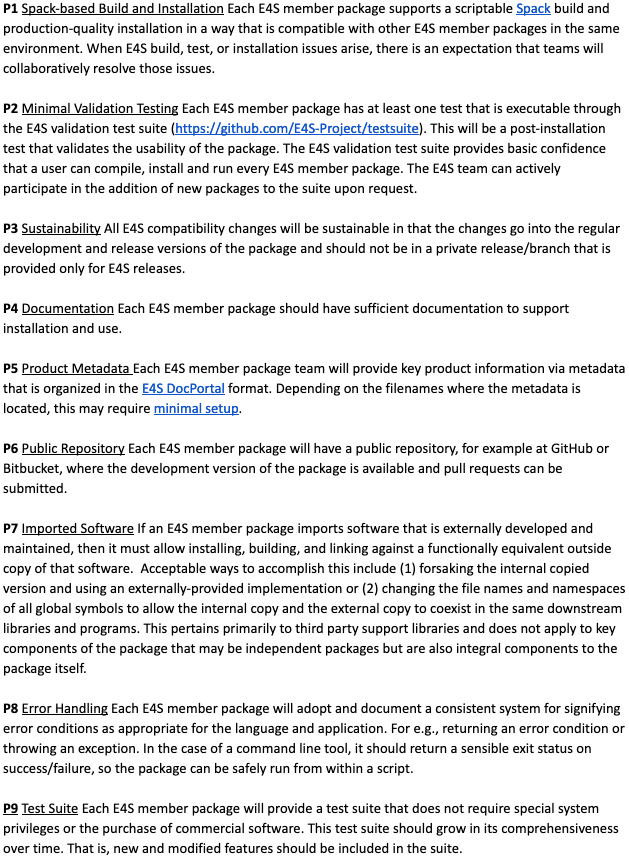
\includegraphics[width=0.9\linewidth]{E4S-Community-Policies-V1}}
        \caption{Version 1 of the E4S community policies. These policies serve as membership criteria for E4S member packages. The E4S community policy effort heavily leveraged the existing xSDK community policies~\cite{xsdk-policies:homepage}.}
          \protect\todo[inline]{Please replace image with higher resolution image so that the image is not blurry or integrate as an editable list.}
        \label{fig:E4S-Community-Policies-V1}
\end{figure}

\begin{figure}
	\centering
	\fbox{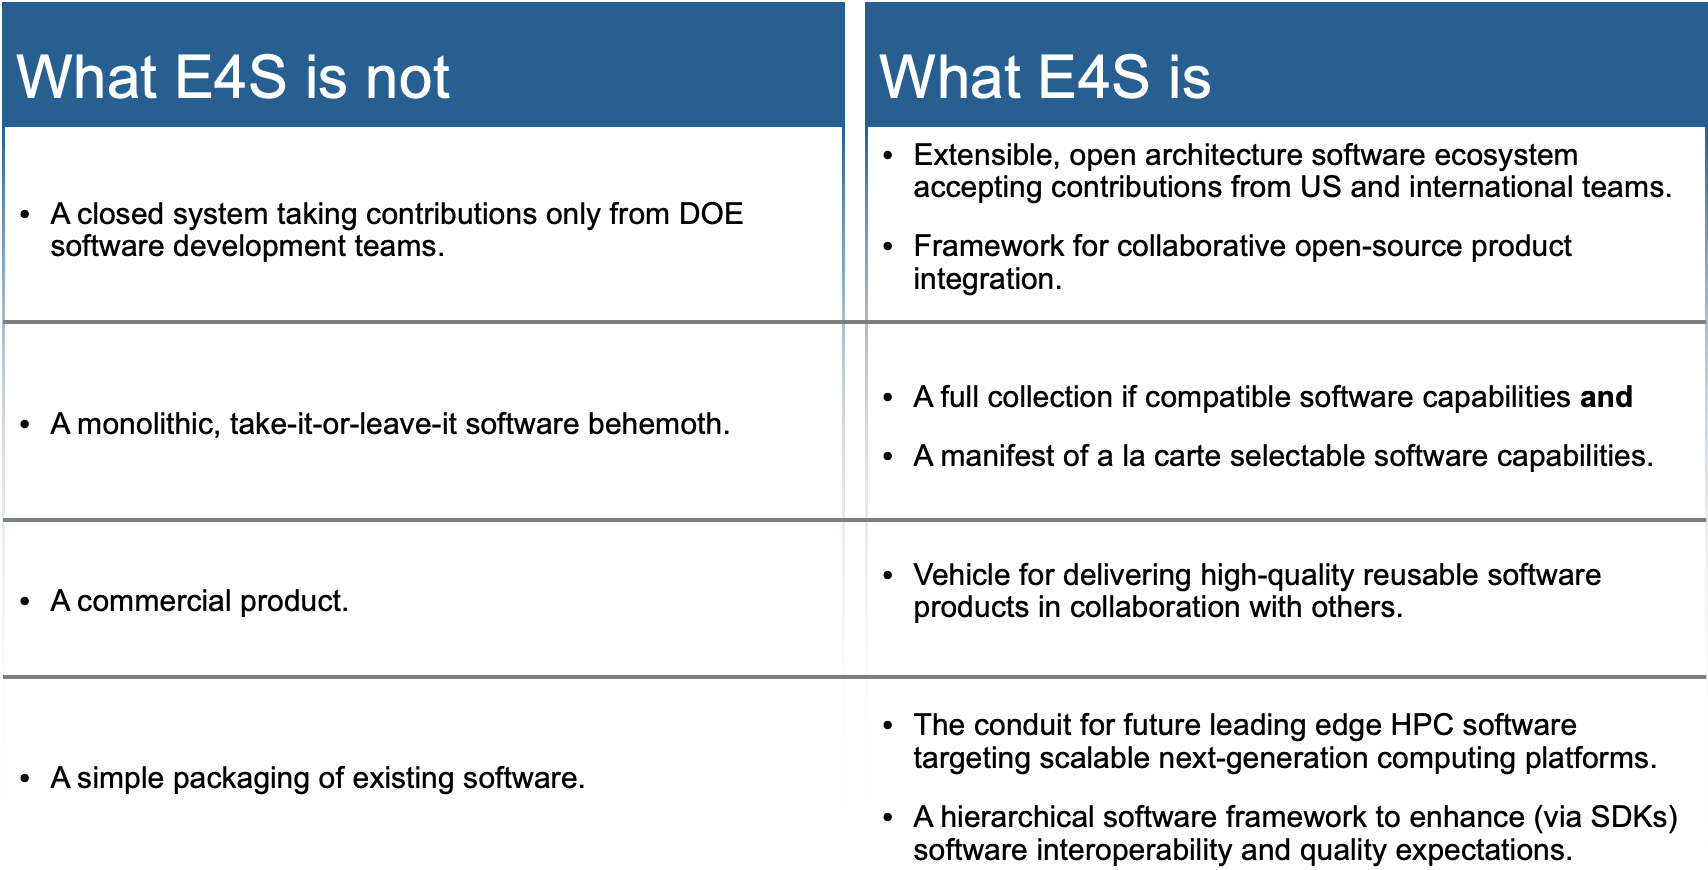
\includegraphics[width=0.9\linewidth]{E4S-Summary}}
	\caption{E4S provides a complete Linux-based software stack that is suitable for many scientific workloads, tutorial, and development environments.  Additionally, it is an open-software architecture that can expand to include any additional and compatible Spack-enabled software capabilities. Because Spack packages are available for many products and easily created for others, E4S is practically expandable to include almost any robust Linux-based product.  Furthermore, E4S capabilities are available as subtrees of the full build. E4S is not monolithic.}
    \protect\todo[inline]{Please make this a table, not a figure, so that it can be edited.}
    \todo[inline]{Please add a ref to this figure (or as a table) in the narrative.}
	\label{fig:e4s-is-isnot}
\end{figure}

\begin{figure}
	\centering
	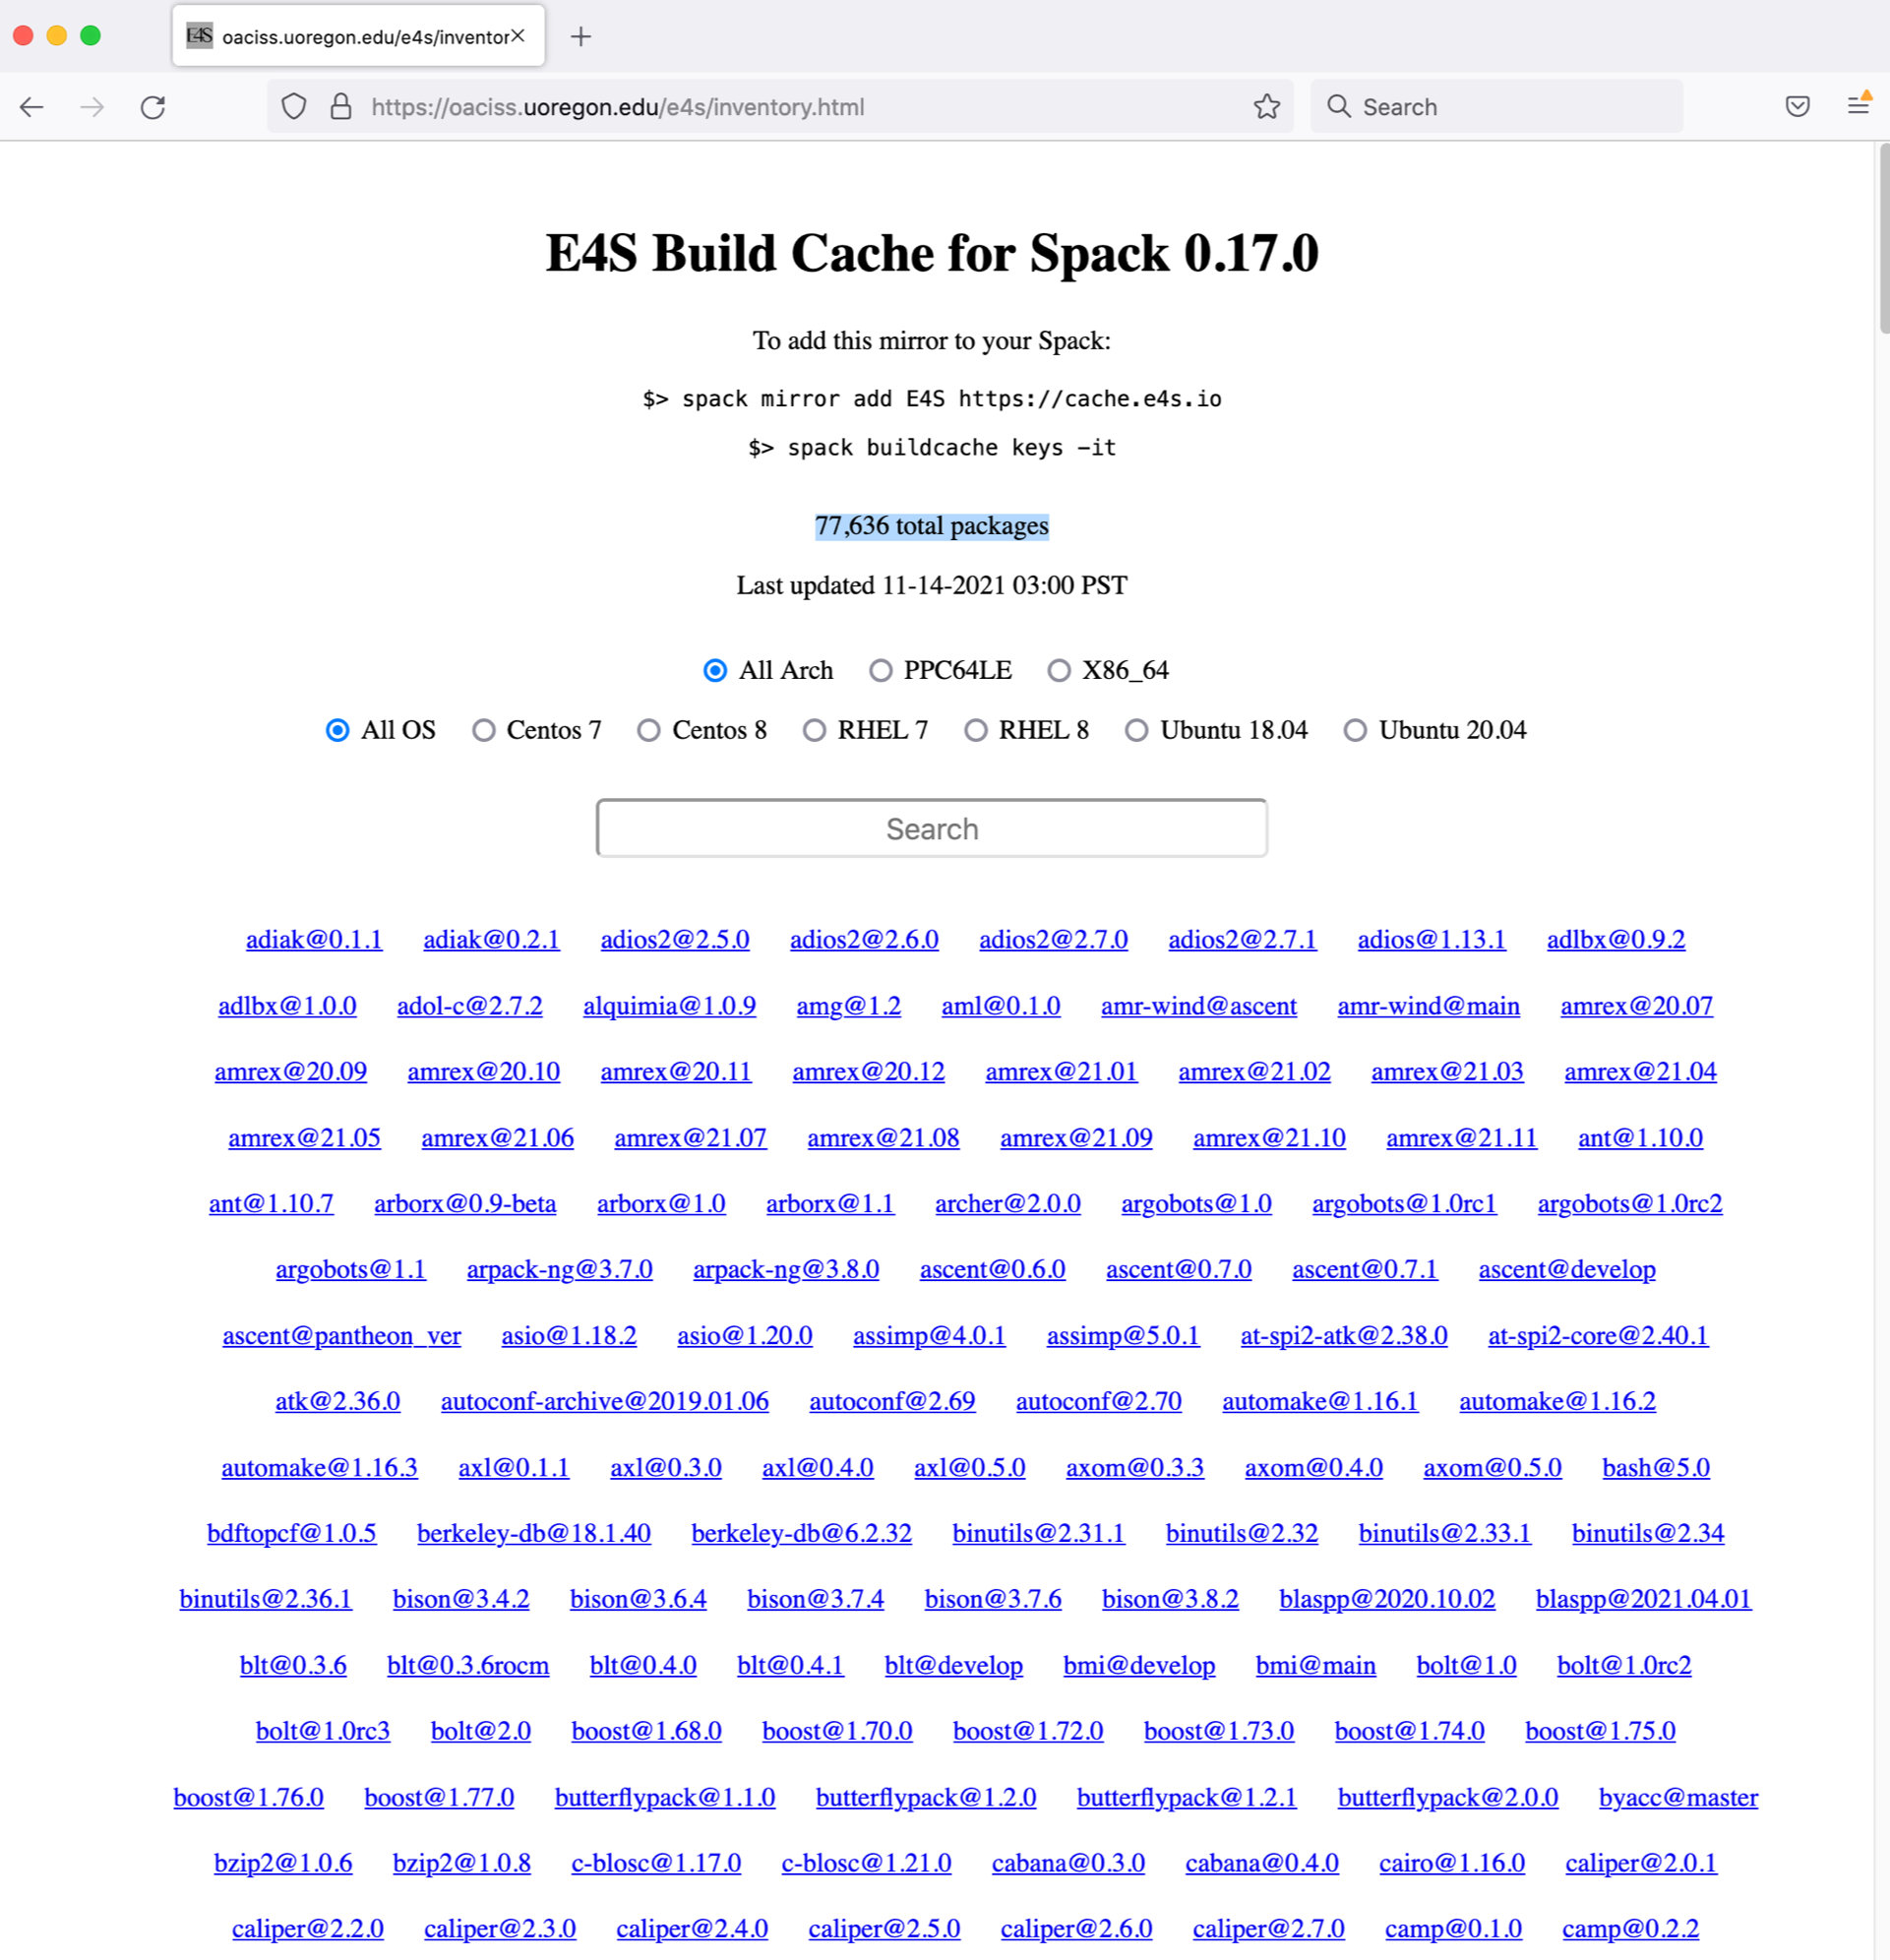
\includegraphics[width=0.9\linewidth]{projects/2.3.5-Ecosystem/2.3.5.01-Ecosystem-SDK/E4S_buildcache_Feb22}
	\caption{Using Spack build cache features, E4S builds can be accelerated via cached binaries for any build signature that Spack has already seen. Between September 2020 and September 2021, more than 31,000 binaries were added to the cache.}
	\label{fig:e4s-build-cache}
	\todo[inline]{Please add a ref to this figure in the narrative.}
\end{figure}

\begin{figure}
	\centering
	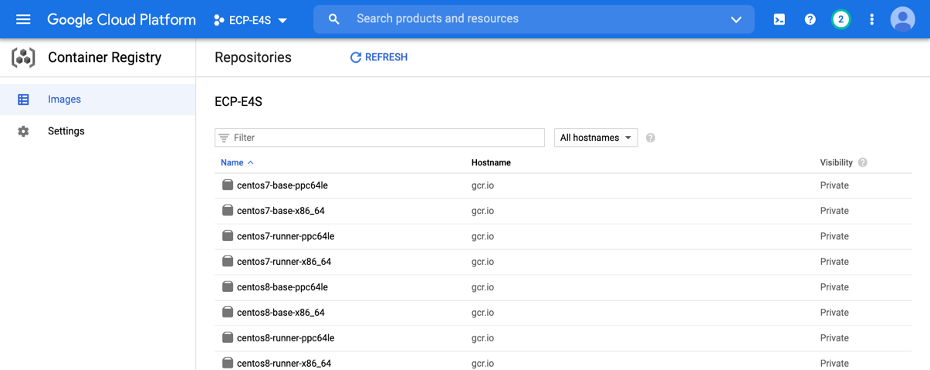
\includegraphics[width=0.9\linewidth]{E4S-GCP}
	\caption{E4S now supports Google Cloud Platform in addition to Amazon Web Services (AWS).}
	\label{fig:e4s-gcp-image}
	\todo[inline]{Please add a ref to this figure in the narrative.}
\end{figure}

The E4S effort is described in further detail in Sections~\ref{subsubsect:sdks} and~\ref{subsect:ecosystem}.

\subsubsection{Software Development Kits}\label{subsubsect:sdks}
One opportunity for a large software ecosystem project such as the ECP ST is to foster increased collaboration, integration, and interoperability among its funded efforts. Part of the ECP ST design is the creation of SDKs.  SDKs are collections of related software products, called \textit{packages}, in which coordination across package teams will improve usability and practices and foster community growth among teams that develop similar and complementary capabilities. SDKs have the following attributes.

\begin{enumerate}
	\item \textbf{Domain scope:} Each SDK will comprise packages whose capabilities are within a natural functionality domain. Packages within an SDK provide similar capabilities that can enable leveraging of common requirements, design, testing, and similar activities. Packages could have a tight complementarity so that ready composability is valuable to the user.
	\item \textbf{Interaction models:} This is how packages within an SDK interact with each other. Packages may be compatible, complementary, and/or interoperable. Interoperability includes common data infrastructure, or the seamless integration of other data infrastructures, and access to capabilities from one package for use in another.
	\item \textbf{Community policies:} These include expectations for how package teams will conduct activities, the services they provide, the software standards they follow, and other practices that can be commonly expected from a package in the SDK.
	\item \textbf{Meta-build system:} This includes robust tools and processes to build from source, install, and test the SDK with compatible versions of each package. This system sits on top of the existing build, install, and test capabilities for each package.
	\item \textbf{Coordinated plans:} Development plans for each package will include efforts to improve SDK capabilities and lead to better integration and interoperability.
	\item \textbf{Community outreach:} Efforts to reach out to the user and client communities will include explicit focus on SDK as a product suite.
\end{enumerate}
	
SDKs provide an aggregation of software products that have complementary or similar attributes. The ECP ST uses SDKs to better ensure product interoperability and compatibility.  SDKs are also essential aggregation points for coordinated planning and testing. SDKs are an integral element of the ECP ST~\cite{Heroux-SDK-Podcast}.  Section~\ref{subsubsect:ecosystem-sdk} describes the six SDK groupings and the current status of the SDK effort.
%\end{table}

\paragraph{ECP ST SDKs}
As part of the delivery of ECP ST capabilities, the team will establish and grow a collection of SDKs. The new layer of aggregation that SDKs represent is important for improving all aspects of product development and delivery. The communities that will emerge from SDK efforts will lead to better collaboration and higher quality products. Established community policies will provide a means to grow SDKs beyond the ECP to include any relevant external effort. The meta-build configurations based on Spack will play an important role in managing the complexity of building the ECP ST software stack by providing a new layer in which versioning, consistency, testing, and build options management can be addressed at a mid-scope below the global build of ECP ST products.
Each of the five ECP ST L3 areas has an SDK project. These projets shepherd five of the six SDKs, along with the products not associated with an SDK. The other SDK, the new Computational Workflows SDK, is overseen by the ExaWorks project. Section~\ref{subsubsect:ecosystem-sdk} provides an update on the progress in defining SDK groupings. For visibility, the same diagram is provided in Figure~\ref{fig:sdk-definition1-0}.

\begin{figure}[htb]
	\centering
	\fbox{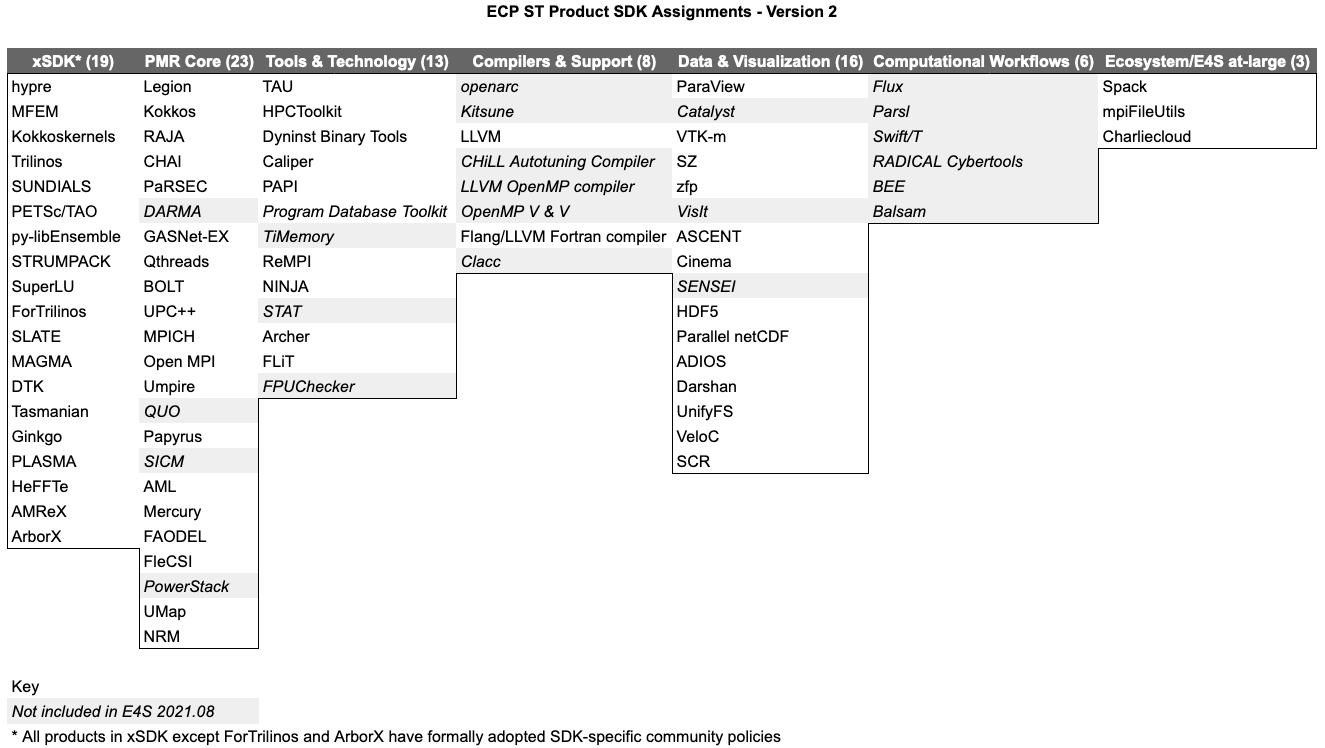
\includegraphics[width=6.5in]{projects/2.3.5-Ecosystem/2.3.5.01-Ecosystem-SDK/SDKdefinitionV2}}
	\caption{\label{fig:sdk-definition1-0}The breakdown of ECP ST products into six SDKs are shown in the first six columns. The rightmost column lists products that are not part of an SDK but are part of the Ecosystem group that will also be delivered as part of the E4S. Section~\ref{subsubsect:ecosystem-sdk} provides an update on the progress in defining SDK groupings.}
\end{figure}


\subsubsection{ECP ST Product Dictionary}\label{subsubsect:dictionary}
In the last year, the ECP has initiated an effort to explicitly manage ECP ST products and their dependencies (Section~\ref{subsubsect:dep-management}).  To eliminate ambiguities, a product dictionary---an official list of publicly named products to which ECP ST teams contribute their capabilities and upon which ECP ST clients depend---is needed.  The ECP product dictionary is one managed table that presently contains 70 primary products and subproducts that are either components within a product or particular implementations of a standard application programming interface (API).  Two special primary products are the Facilities stack and Vendor stack.  Having these stacks on the list enables ST teams to indicate that the team's capabilities are being delivered to ecosystems outside of the ECP.

Figure~\ref{fig:product-dictionary-overview} describes the policy for ECP ST teams to add and manage their contributions to the product dictionary.  Figure~\ref{fig:product-dictionary} shows a snapshot of the beginning and end of the current \textit{ECP ST Product Dictionary}, which is maintained on the ECP Confluence wiki. \todo{Is ``wiki" how it is listed in this document? If so, leave it. If not, please remove. Please make the same change in the caption of Figure 14.}

\begin{figure}
	\centering
	\fbox{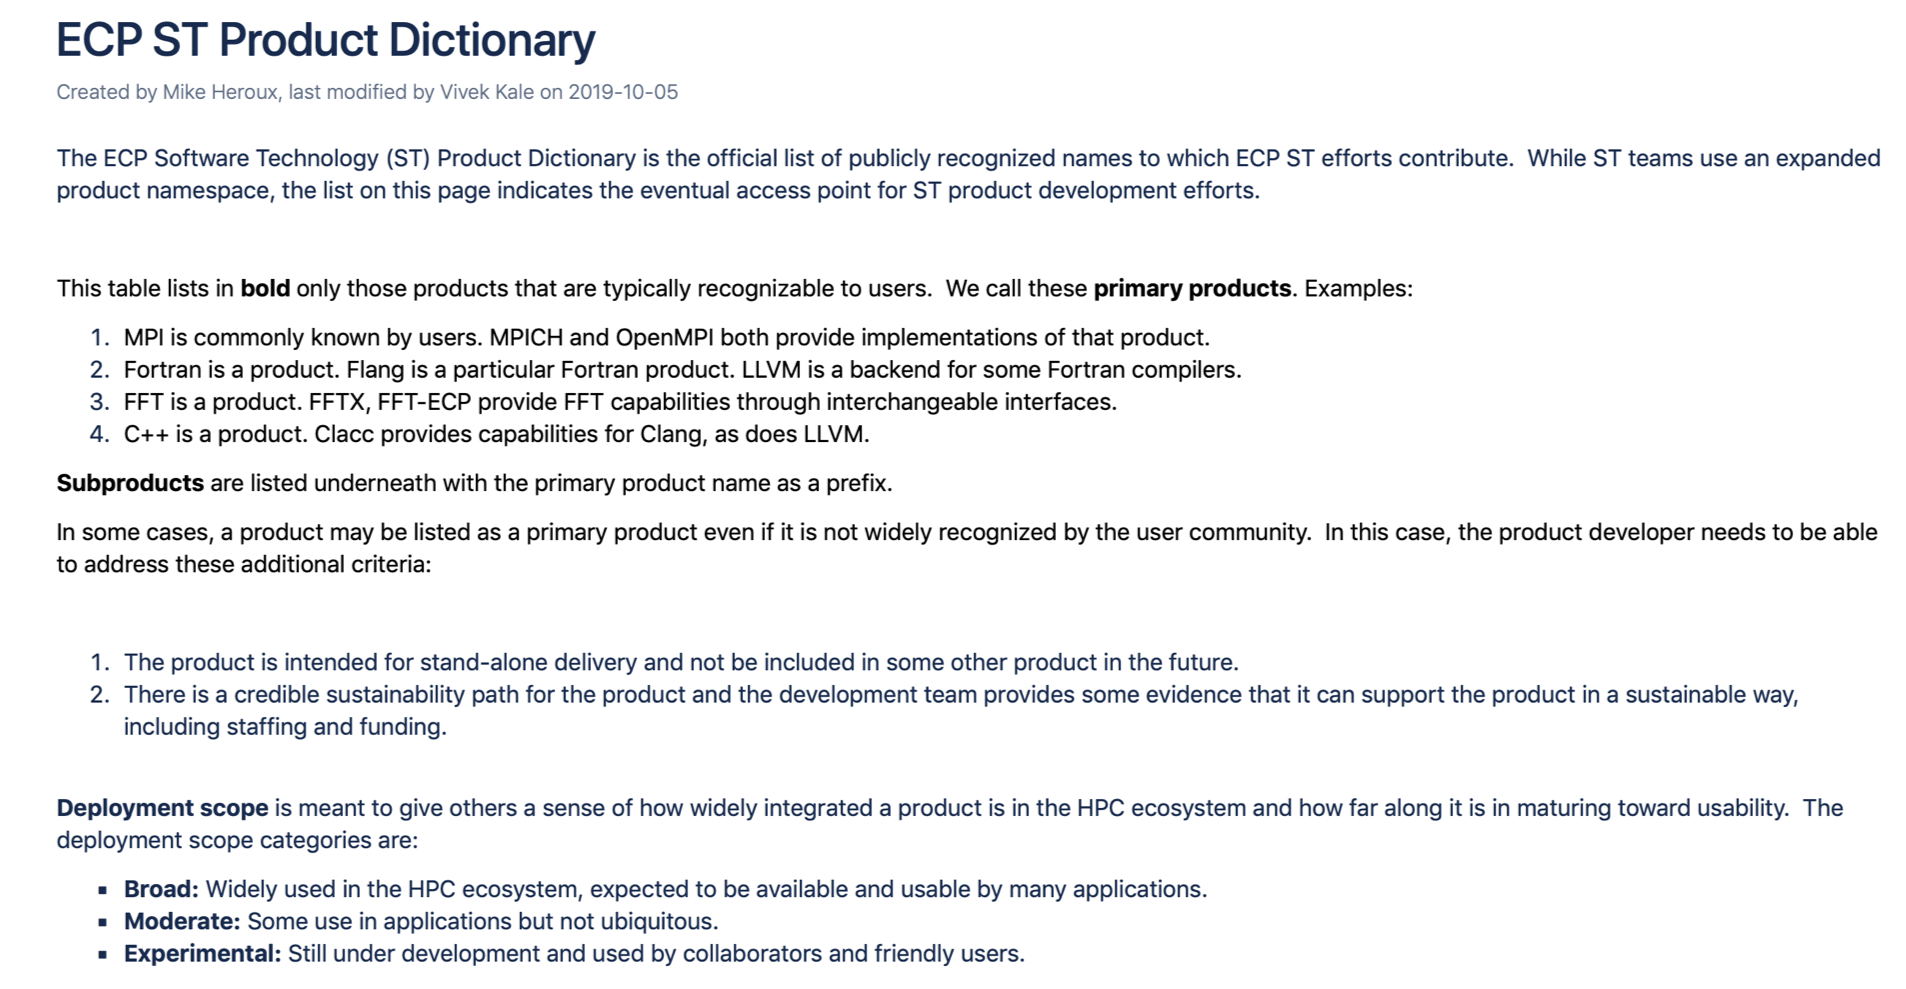
\includegraphics[width=0.9\linewidth]{ProductDictionaryOverview}}
	\caption{Screenshot from the top of the ECP Confluence wiki page containing the \textit{ECP ST Product Dictionary}.  The product dictionary structure contains primary and secondary products.  Client (i.e., consumer) dependencies are stated against the primary product names only, enabling unambiguous mapping of AD-on-ST and ST-on-ST dependencies.}
	\label{fig:product-dictionary-overview}
\end{figure}

\begin{figure}
	\centering
	\fbox{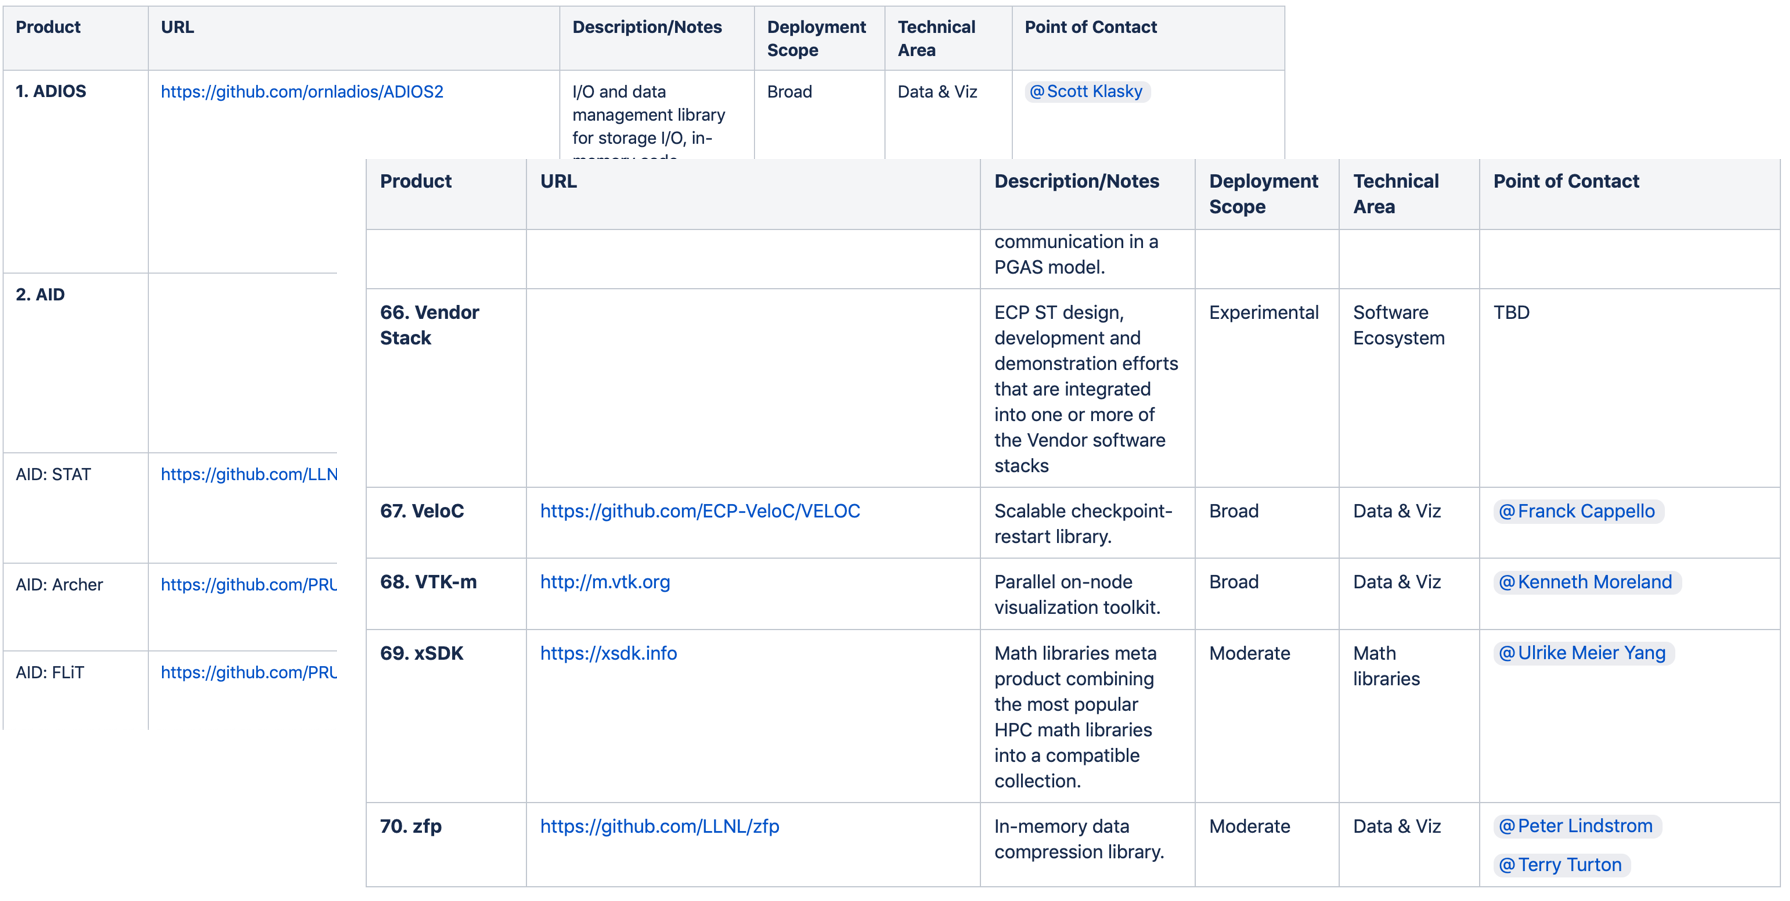
\includegraphics[width=0.9\linewidth]{ConfluenceProductDictionaryExample}}
	\caption{Screenshots of the \textit{ECP ST Product Dictionary} table.  The table is actively managed to include primary and secondary products to which the ECP ST team contributes and upon which ECP ST clients depend.  Presently, the product dictionary contains 70 primary products.  Secondary products are listed under the primary product with the primary product as a prefix.  For example, AID is the second primary product in the table shown here.  STAT, Archer, and FLIT are component subproducts.  MPI (not shown) is another primary product.  MPICH and OpenMPI are two robust MPI implementations and are listed as MPI subproducts.}
	\label{fig:product-dictionary}
\end{figure}

\subsubsection{ECP Product Dependency Management}\label{subsubsect:dep-management}
Given the \textit{ECP ST Product Dictionary} and a similar dictionary for ECP AD and co-design products, the ECP has created a dependency database that enables the creation and characterization of product-to-product dependencies. The ECP manages these dependencies in a Jira database by using a custom Jira issue type: Dependency.  The dependency database provides an important tool for understanding and managing ECP activities.  The dependency information is valuable within and outside the project.  Figure X \todo{Add figure number in place of X} shows a screenshot of the Jira dependency database dashboard, and Figure X \todo{Add figure number in place of X} shows a screenshot of an example query result in the Jira dependency database.

\begin{figure}
	\centering
	\fbox{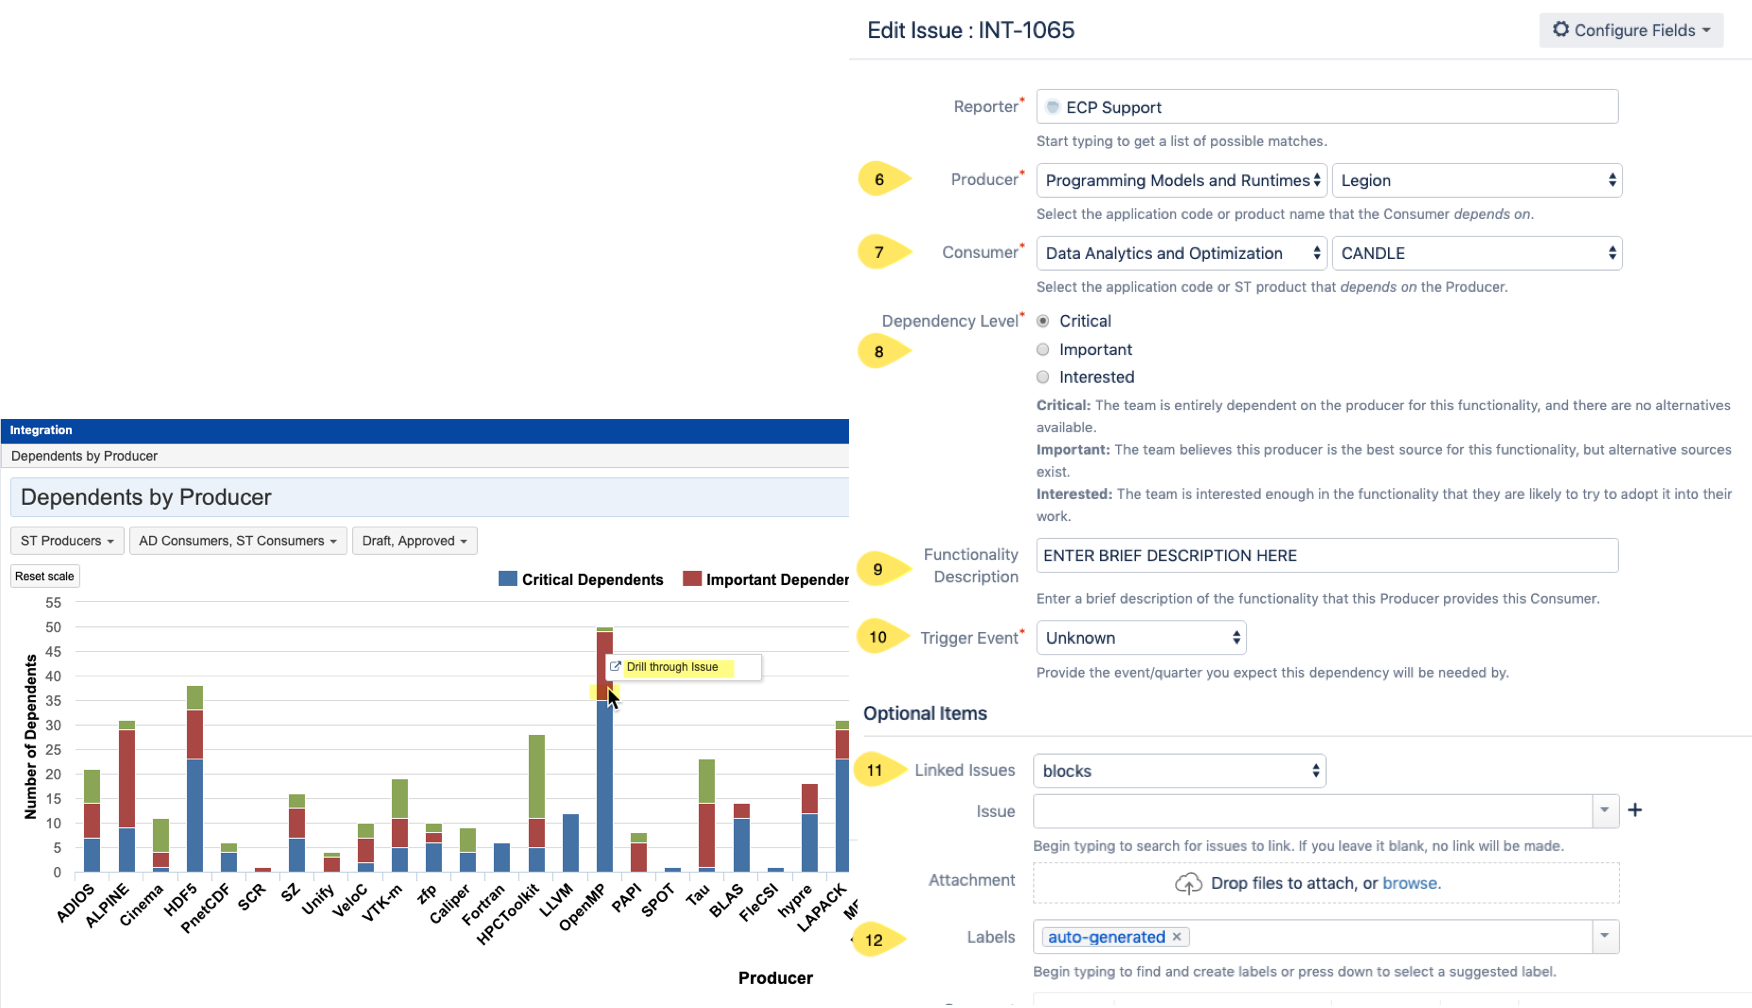
\includegraphics[width=0.9\linewidth]{DependencyDashboard-EditPanel}}
	\caption{Using Jira, the ECP manages its AD, ST, HI, vendor, and facilities dependencies.  This figure shows a screenshot of the Jira dependency database dashboard and an edit panel, which supports the creation and management of a consumer-on-producer dependency.}
	\label{fig:dependency-dashboard-edit}
	\todo[inline]{Please add a ref to this figure in the narrative.}
\end{figure}

\begin{figure}
	\centering
	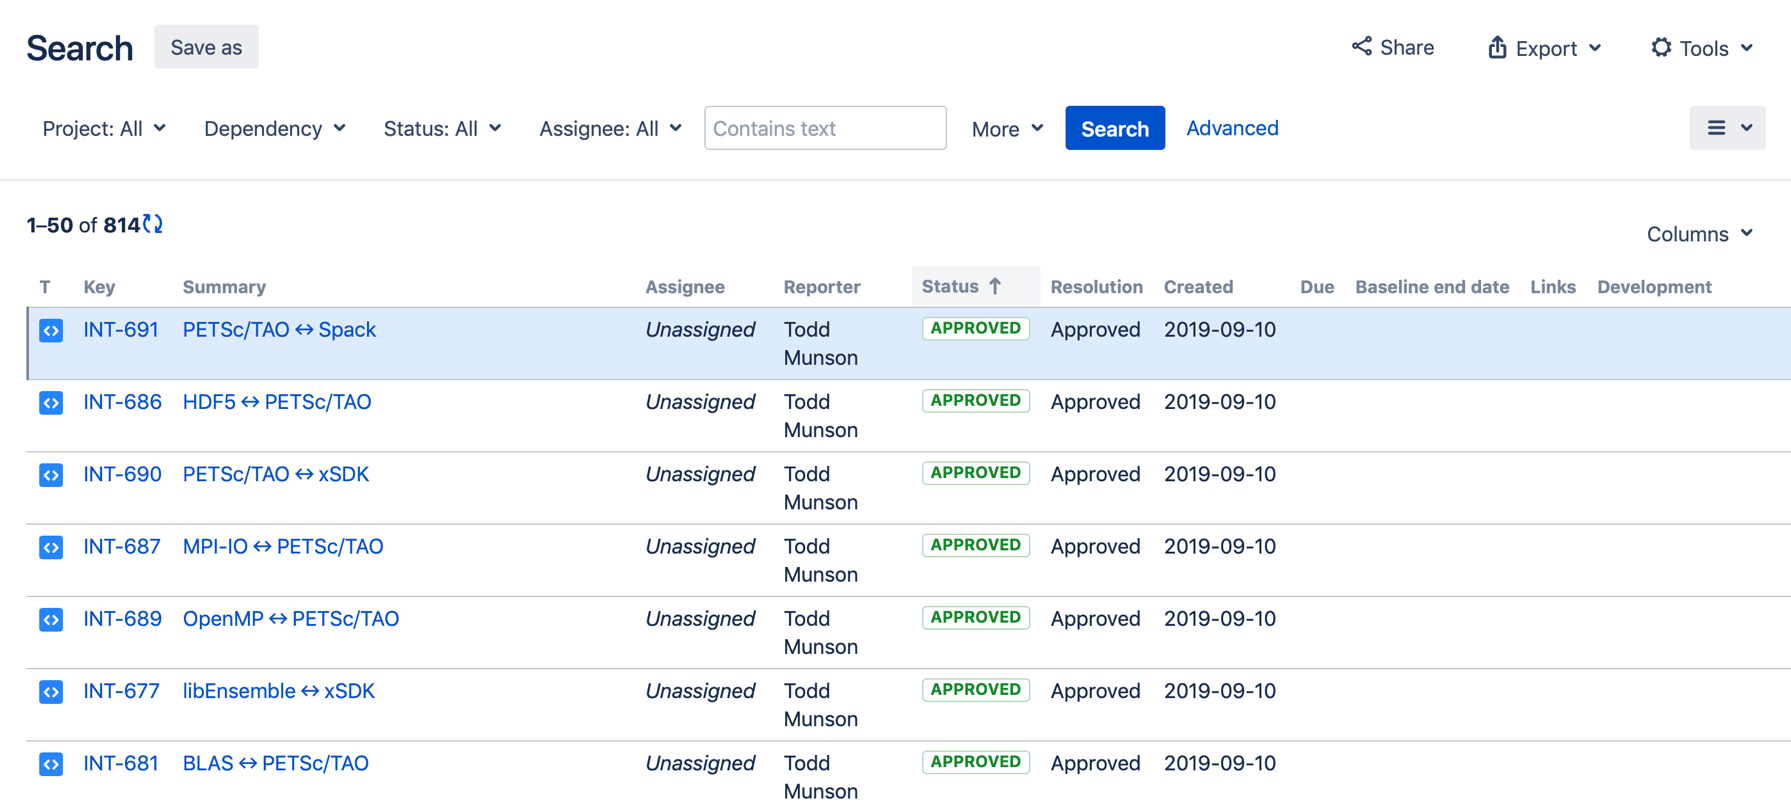
\includegraphics[width=0.9\linewidth]{PETSc-TAO-Dependencies}
	\caption{This query result from the ECP Jira dependency database lists all consumers of capabilities from the PETSc/TAO product. Selecting the details of one of the dependency issues shows how critical the dependency is and any custom information peculiar to the particular dependency.}
	\label{fig:petsc-tao-dependencies}
	\todo[inline]{Please add a ref to this figure in the narrative.}
\end{figure}

\newpage
\subsection{ECP ST Planning and Tracking}

Although the ECP is an official 413.3B federal construction project using an earned value management system, the ECP is permitted to tailor the planning process to obtain the flexibility needed for a software project, the requirements of which are emerging as the project proceeds.  This section describes how the ECP ST plans activities using the Jira project management tool.  The following sections discuss P6 activities, which are similar to milestones, and KPP-3, which is associated with the ECP ST.


\subsubsection{ECP ST P6 Activity Issues}

ECP ST uses a custom Jira issue type called \textit{P6 Activity}.  Each L4 subproject creates a series of P6 activity issues that extend to the end of the ECP (Q3 FY23).  Except for the current fiscal year, one P6 Activity issue describes expected deliverables as a planning package.  Six months before the start of a fiscal year, the planning package for the coming year is replaced with four to six issues that span the year with baseline start and end dates, an estimate of the percent annual budget and a high-level description.  Eight weeks before the start of an activity, full details about staffing, completion criteria, and more are added to the issue.  Figure~\ref{fig:planning-process} shows the steps in diagram form.  

Cost, scope, and schedule for the ECP ST are tracked and managed by monitoring the progress of the collection of P6 Activities.  Value is accrued when a P6 Activity issue is marked ``Done'' in the Jira database.  Schedule and cost performance indices are derived from the status of the P6 Activities.  Schedule, cost, and scope changes against the plan are managed via a formal project change request process.

\begin{figure}
	\centering
	\fbox{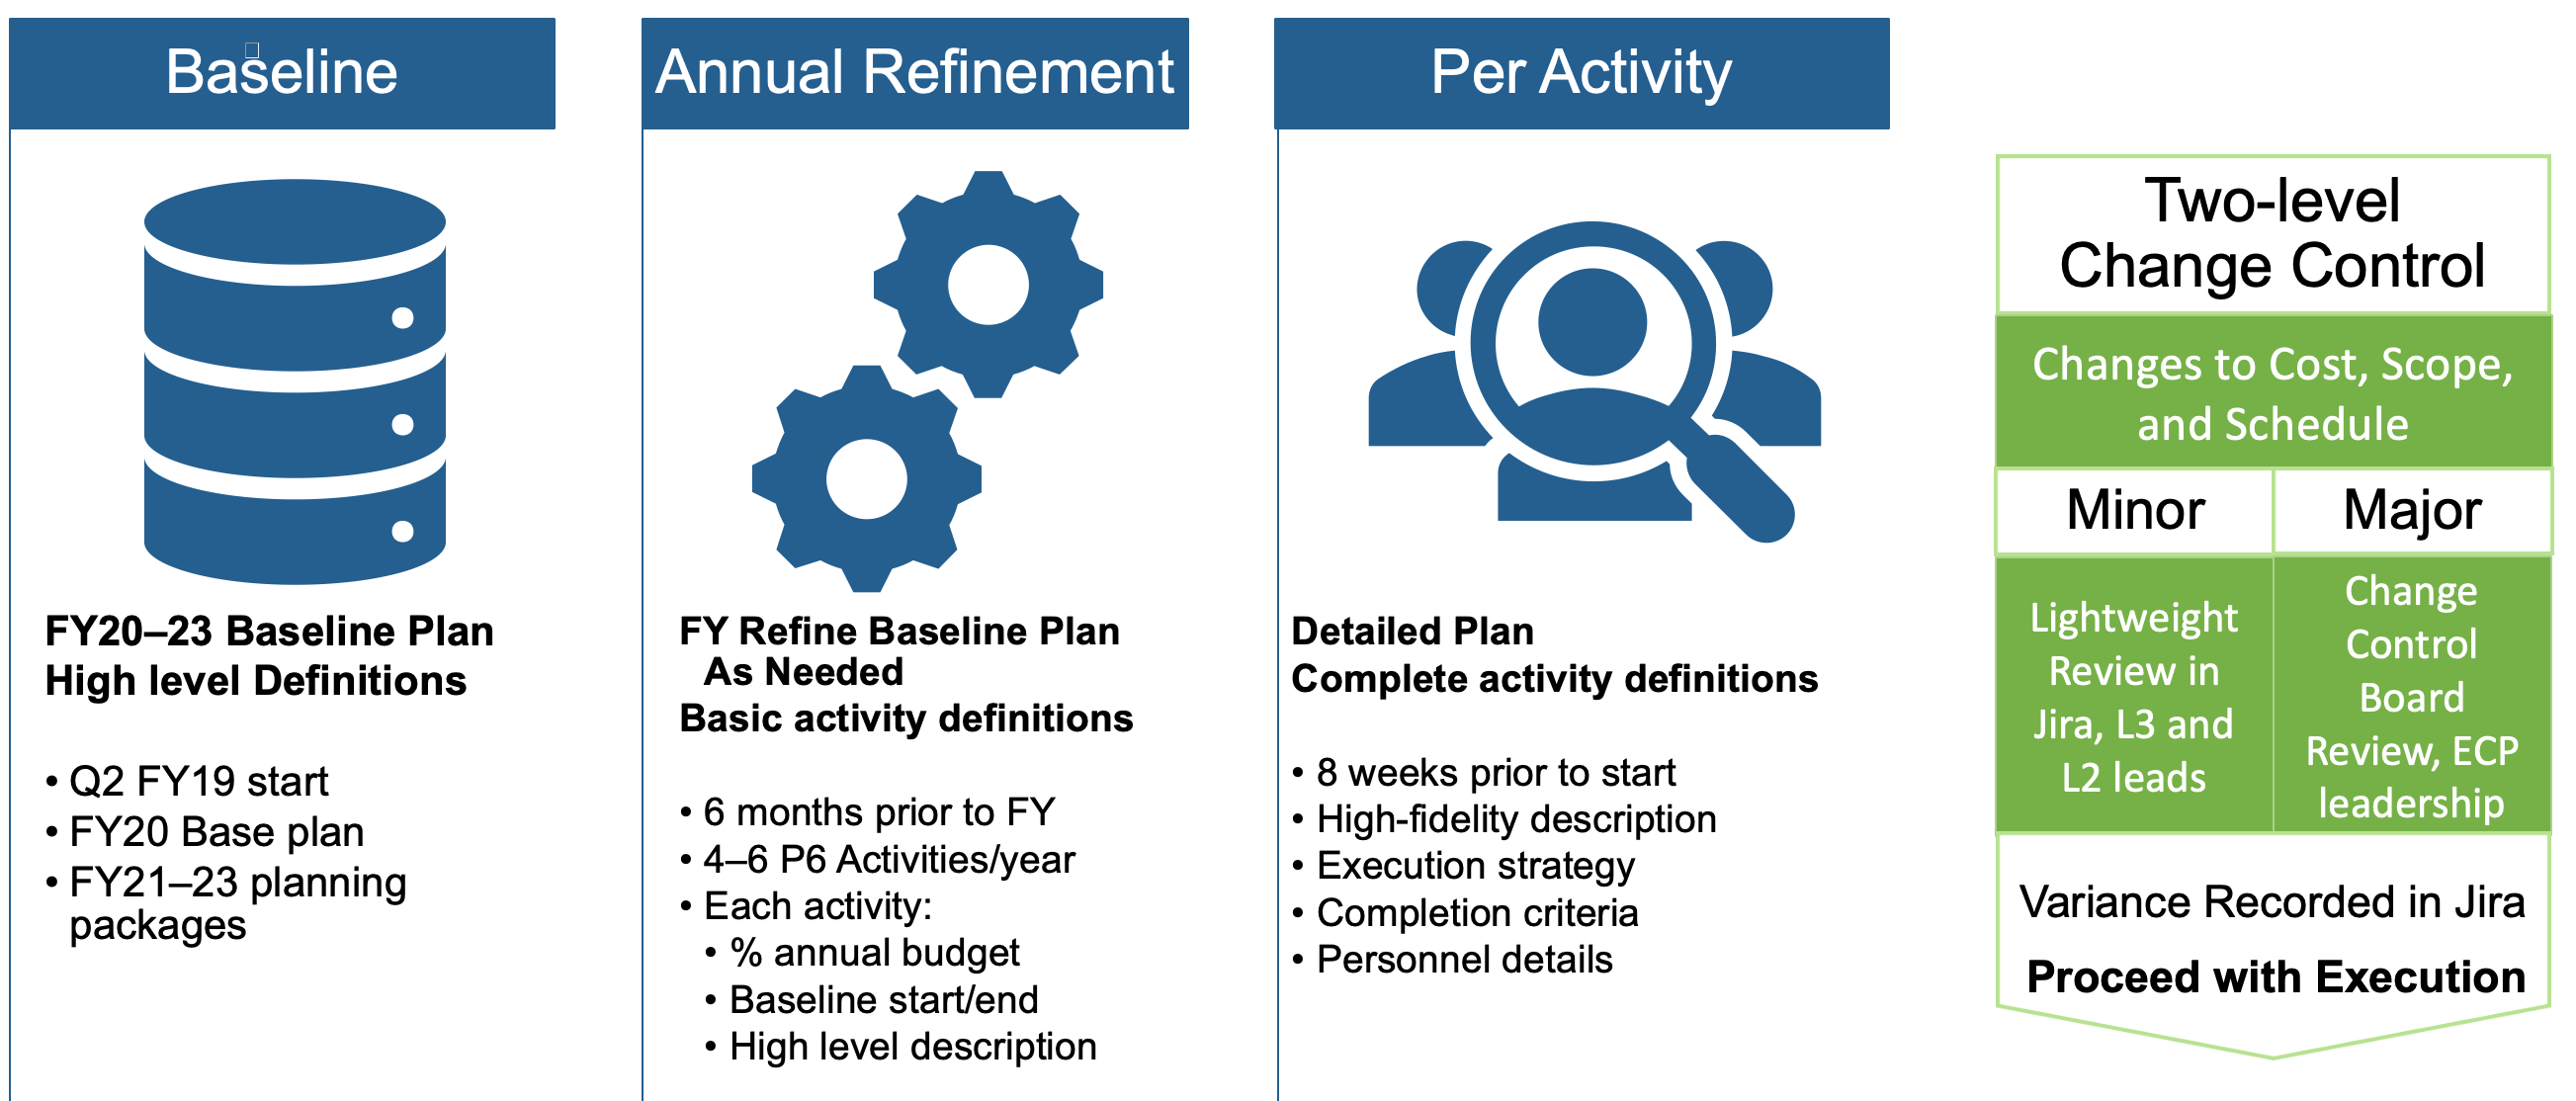
\includegraphics[width=0.9\linewidth]{Planning-Process}}
	\caption{Example of a P6 Activity.} 
	\protect\todo[inline]{The former caption was just repeating verbatim the previous paragraph. Please add a caption that describes what is shown in the image.}
	\label{fig:planning-process}
\end{figure}


\subsubsection{KPP-3}

The ECP has four KPPs.  Figure~\ref{fig:kpp-definitions} shows the KPP definitions. KPP-3 focuses on a productive and sustainable software ecosystem. The ECP ST is the primary owner of this KPP along with co-design projects in the ECP AD.  The focus of KPP-3 is to define and track capability integrations of ST products into the client environment, as described in this section. 

\begin{figure}
	\centering
	\fbox{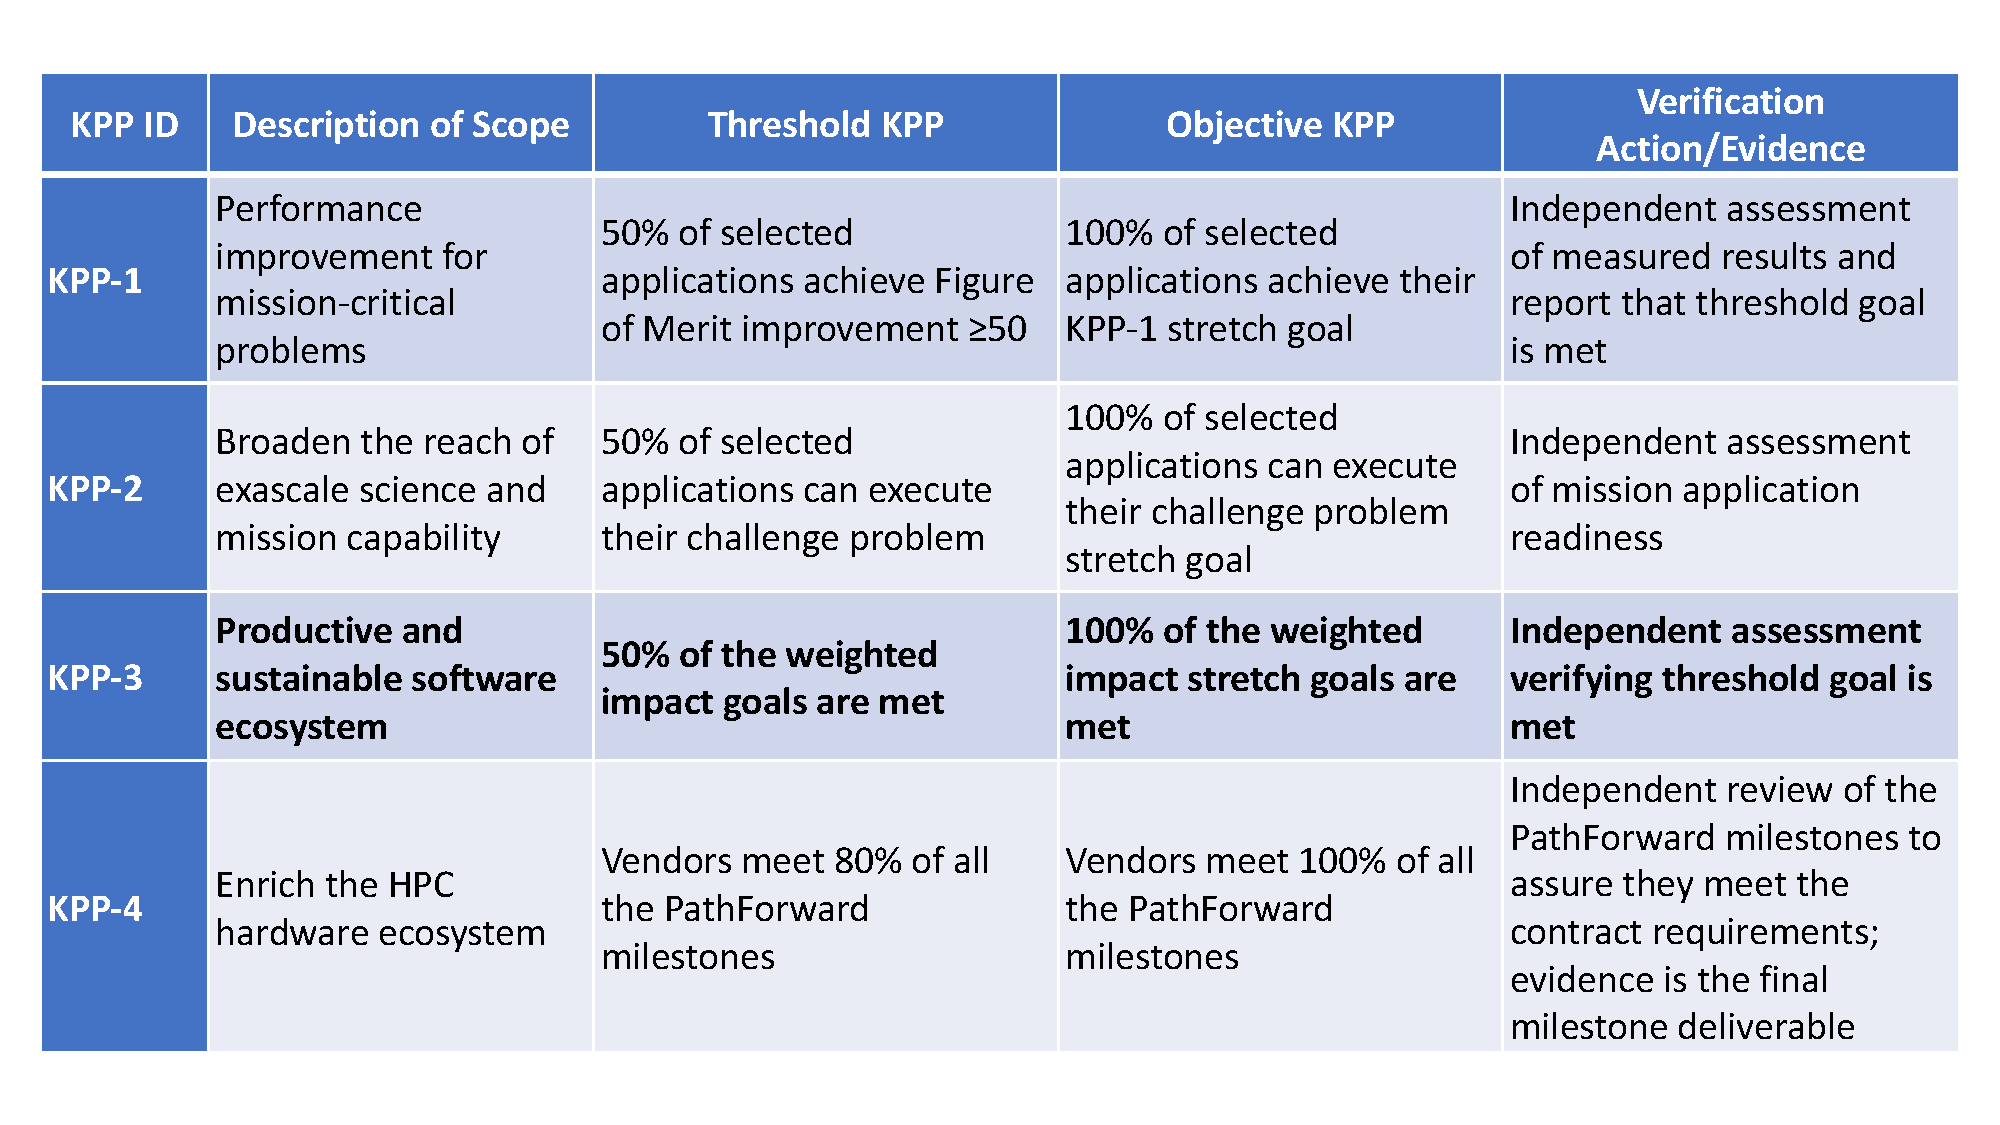
\includegraphics[width=0.9\linewidth]{KPP-Definitions}}
	\caption{The ECP's four KPPs.}
	\label{fig:kpp-definitions}
	\todo[inline]{Please convert this to an editable table or provide a higher-resolution version without blurry text.}
\end{figure}



The following terms are defined for clarity.
\begin{itemize}
	\item \textbf{Capability:} Any significant product functionality, including existing features adapted to the pre-exascale and exascale environments, that can be integrated into a client environment.
	\item \textbf{Integration goal:} A statement of impact on the ECP ecosystem in which a software capability is used in a consequential and sustainable way by a client in pre-exascale environments first, then in exascale environments.  Integration goals are product focused.  A project that contributes to more than one product will have a KPP-3 Jira issue for each of its products.
	\item \textbf{Integration score: }The number of successful capability integrations into a client environment (Table~\ref{table:KPP-3-scoring}).
	\item \textbf{Sustainable:} For KPP-3, \textit{sustainable} means that the capability is integrated in a way that reasonably ensures future use of the capability beyond the end of the ECP.  For libraries, \textit{sustainable} generally means that library usage is made from the source code in the main repository and use of the library is tested regularly as a part of the client code's regular regression testing.  For tools, \textit{sustainable} generally means that the tool is available as needed in the exascale environment.  For prototype capabilities that are incorporated into vendor and community software, the impact of the prototype is still visible to subject matter experts (SMEs).
\end{itemize}

\paragraph{Defining an Integration Goal:}
Integration goals are defined per product within each project.  The goal statement will include the following.
\begin{itemize}
	\item The name of the product to which the project contributes.  The product must be listed in the \textit{ECP ST Product Dictionary}.
	\item A description of the target clients' environments into which the product capabilities will be integrated.  Specific clients can be listed but are not necessary.  Clients must be part of the ECP or otherwise part of the exascale systems ecosystem, such as a vendor or facility partner.   
	\item A general description of the nature of the integration that addresses what it means to be successfully integrated.
\end{itemize}

\begin{table}[h!]
	\begin{tabular}{|L{1.5in}|L{2.0in}|L{2.5in}|}\hline
		\rowcolor{LightCyan}
		Integration score & Capability & Integration description\\\hline
		One point per capability sustainably integrated by a client per exascale platform used. &
		Complete, sustainable integration of a significant product capability into a client environment in a pre-exascale environment (tentative score) and in an exascale environment (confirmed score). &
		Clients acknowledge benefit from product capability use and considers it part of their workflow. Integration is sustainable with documentation and testing. Integration of product capability into main product repo and SDK/E4S environments is completed.\\\hline
	\end{tabular}
	\caption{\label{table:KPP-3-scoring} Integration goal scoring. One point is accrued when a client integrates and sustainably uses a product's capabilities.  Scores are assessed annually.}
\end{table}


\paragraph{Demonstrating and Recording Progress toward an Integration Goal:}
All artifacts and evidence of progress will be captured in the Jira KPP-3 issue associated with a product integration goal as progress is made.  All integration scores are tentative until the capability is available and demonstrated in exascale environments.  Table~\ref{table:KPP-3-values} summarizes the defined values.

\begin{table}[h!]
	\begin{tabular}{|L{0.6in}|L{2.0in}|L{3.4in}|}\hline
		\rowcolor{LightCyan}
		Value & Definition & Description\\\hline
		Present & The current integration score. & This is always an indication of the progress that the team has made. The present value is assessed annually.\\\hline
		Passing & The minimum integration score required for the product to be counted as part of ECP ST progress toward KPP-3. & The passing score is between 4 and 8 for each integration goal, in which 4 is for larger integration efforts, and 8 is for smaller ones. This is equivalent to accomplishing one to two capability integrations per year, per product.\\\hline
		Stretch & The maximum reasonably achievable integration score for a product if capability integrations are successful with all potential ECP clients.   & The stretch value shows the overall integration potential.\\\hline
	\end{tabular}
	\caption{\label{table:KPP-3-values} Key metric values. These values are determined by the L4 subproject team when defining its KPP-3 issue.}
\end{table}

\paragraph{Assessment Process:}
Although progress is recorded as it is achieved, progress assessment is done annually, including input from external SMEs.  ECP leadership and SMEs will review integration score evidence, confirming or adjusting integration scores.
Assessments can result in a reduced integration score from a previous year if a client has stopped using a capability that was previously used.

\paragraph{Transition from Tentative to Confirmed Integration Score:}
Each integration score is tentative until the capability is available and demonstrated to be effective in the exascale environments.  Demonstration can be achieved in a variety of ways so that ECP leadership and SMEs are reasonably certain that the capability positively impacts the client in exascale environments.  At this point, the integration score becomes confirmed. 
Typically, the transition from tentative to confirmed would be a low-cost, independent demonstration or accomplished within the client’s environment as the client is conducting its own assessments. 
The planned exascale system, El Capitan, that can support National Security Applications will not be available until the end of FY23. Integrating ST products into National Security Applications will be considered for transition from tentative to confirmed when: (1) evidence of integration is provided during FY20--22 ASC L1 and L2 milestones related to ECP/ATDM National Security Application readiness for exascale platforms and/or (2) integration is demonstrated on the El Capitan early access systems and exercises capabilities similar to those anticipated to be important for effectively using El Capitan.  For KPP-3 capability integrations targeted at El Capitan, the ECP will use the best available confirmation process in FY23. Table~\ref{table:KPP-3-impact} explains the weight of the integration scores. 


\begin{table}[h!]
	\begin{tabular}{|L{1.0in}|L{0.5in}|L{4.5in}|}\hline
		\rowcolor{LightCyan}
		Impact level & Weight & Comments\\\hline
		High & 2 & The score for integration goals associated with high-impact products will be added to the KPP-3 score with a weight of 2.\\\hline
		Normal & 1 & Most KPP-3 Jira issues will have a weight of 1.\\\hline
		Risk mitigating & 0.5 & Some KPP-3 Jira issues are associated with products that help plan for the potential risks if high-impact products do not deliver as expected.\\\hline
		Shared  & 0.5 & Some projects receive funding from both NNSA and DOE SC (e.g., RAJA/Kokkos). For these projects, the score is balanced to reflect dual contributions.\\\hline
	\end{tabular}
	\caption{\label{table:KPP-3-impact} Integration scores. Each integration score will have an associated weight, depending on the potential impact if integration targets are not met.}
\end{table}

The KPP-3 score is the weighted sum of all integration goals that have an integration score that meets or exceeds its passing value. 
The KPP-3 score will initially be tentative.  The KPP-3 score is not officially met until the weighted sum of confirmed integration scores exceeds 50\% of the total possible points.


\subsubsection{ECP ST Software Delivery}
One essential activity for---and the ultimate purpose of---ECP ST is the delivery of a software stack that enables productive and sustainable exascale computing capabilities for target ECP applications and platforms and the broader HPC community. The ECP ST Software Ecosystem and Delivery sub-element (WBS 2.3.5), and the SDKs in each sub-element, provide the means by which the ECP ST will deliver its capabilities.
\paragraph{ECP ST Delivery and HI Deployment:}
Providing the ECP ST software stack to ECP applications requires coordination between the ECP ST and ECP HI. The focus areas have a complementary arrangement in which the ECP ST delivers its products, and the ECP HI deploys them. The process is described specifically as follows.
\begin{itemize}
	\item The ECP ST delivers software.  ECP ST products are delivered directly to application teams, vendors, and facilities.  The ECP ST designs and implements products to run on DOE computing facilities platforms and make products available as source code via GitHub, GitLab, or another accessible repository.
	\item The ECP HI facilitates efforts to deploy ST and other software on facilities platforms by installing them where users expect to find them. This could be in \texttt{/usr/local/bin} or a similar directory or available via ``module load.''
\end{itemize}
Separating the concerns of delivery and deployment is essential because these activities require different skill sets. Furthermore, the ECP ST delivers its capabilities to an audience that is beyond the scope of specific facilities’ platforms. This broad scope is essential for the sustainability of ECP ST products, expanding the user and developer communities needed for vitality. Additionally, the ECP HI, computer system vendors, and other parties provide deployable software outside the scope of the ECP ST, thus having the critical skills needed to deploy the entire software stack.

\paragraph{ECP ST Delivery Strategy:}
The ECP ST delivers its software products as source code, primarily in repositories found on GitHub or GitLab installations or similar platforms. Clients such as the ECP HI, OpenHPC, and application developers with direct repository access then take the source and build, install, and test the ECP ST software. The delivery strategy is outlined in Figure~\ref{fig:hierarchy}, and  
%
users access ECP ST products using the following basic mechanisms.
\begin{itemize}
	\item \textbf{Build from source code:} Most ECP ST products reach at least some of their user base via direct source code download from the product repository.  In some cases, users download one compressed file that contains the product source, then expand the file to expose the collection of source and build files.  Increasingly, users will fork a new copy of an online repository.  After obtaining the source, users execute a configuration process that detects local compilers and libraries and then builds the product.  This kind of access can be a barrier for some users because users need to build the product and can encounter a variety of challenges in that process, such as an incompatible compiler or a missing third-party library that must first be installed.  However, building from the source can be a preferred approach for users who want control over compiler settings or want to adapt how the product is used (e.g., turning on or off optional features, creating adaptations that extend product capabilities). For example, large library frameworks, such as PETSc and Trilinos, have many tunable features that can benefit from users building from source code.  Furthermore, these frameworks support user-defined functional extensions that are easier to support when users builds the product from source. The ECP ST is leveraging and contributing to the development of Spack~\cite{gamblin+:sc15}.  Via metadata stored in a Spack package defined for each product, Spack leverages a product's native build environment, along with knowledge about its dependencies, to build the product and dependencies from source.  Spack plays a central role in ECP ST software development and delivery processes by supporting turnkey builds of the ECP ST software stack for the purposes of continuous integration testing, installation, and seamless multiproduct builds.
	\item \textbf{DOE computing facilities:} Each DOE computing facility---Argonne Leadership Computing Facility (ALCF), Oak Ridge Leadership Computing Facility (OLCF), National Energy Research Scientific Computing Center (NERSC), LLNL, and the Atmosphere, Climate, and Ecosystem Science (ACES) collaboration (Los Alamos National Laboratory [LANL] and Sandia National Laboratories~[SNL]) provides pre-built versions of 17--20 ECP ST products, although the exact mix of products varies somewhat at each site. Many of these products are what users would consider to be part of the core system capabilities, including compilers---such as Flang (Section~\ref{subsubsect:flang}) and LLVM (Section~\ref{subsubsect:sollve})---and parallel programming environments, such as MPICH (Section~\ref{subsubsect:mpich}), OpenMPI (Section~\ref{subsubsect:openmpi}), and OpenMP (Section~\ref{subsubsect:bolt}).  Development tools, such as PAPI (Section~\ref{subsubsect:exapapi}) and TAU (Section~\ref{subsubsect:tau}), are often part of this suite if they are not already included in the vendor stack. Math and data libraries, such as PETSc (Section~\ref{subsubsect:petsc}), Trilinos (Section~\ref{subsubsect:peeks}), HDF5 (Section~\ref{subsubsect:exahdf5}), and others are also available in some facilities' software installations. The team anticipates and hopes for increased collaboration with facilities via the ECP HI focus area.  The team is also encouraged by multi-lab efforts, such as the Tri-Lab Operating System Stack (TOSS)~\cite{TOSS}, that are focused on improving the uniformity of software stacks across facilities.
	\item \textbf{Vendor stacks:} Computer system vendors leverage DOE investments in compilers, tools, and libraries.  Of particular note is the wide use of MPICH~(Section~\ref{subsubsect:mpich}) as a software base for most HPC vendor MPI implementations and the requirements, analysis, design, and prototyping that ECP ST teams provide.  Section~\ref{subsection:external-contributions} describes some of these efforts.
	\item \textbf{Binary distributions:} Approximately 10 ECP ST products are available via binary distributions, such as common Linux distributions, particularly via OpenHPC~\cite{OpenHPC}. The ECP ST intends to foster the growth of availability via binary distributions as an important way to increase the size of the user community and improve product sustainability via this broader user base.  
	\item \textbf{Container and cloud environments:} E4S is available via an increasing number of container and cloud environments, such as Docker, Shifter, Singularity, CharlieCloud, AWS, and Google Cloud.
\end{itemize}

\begin{figure}
	\centering
	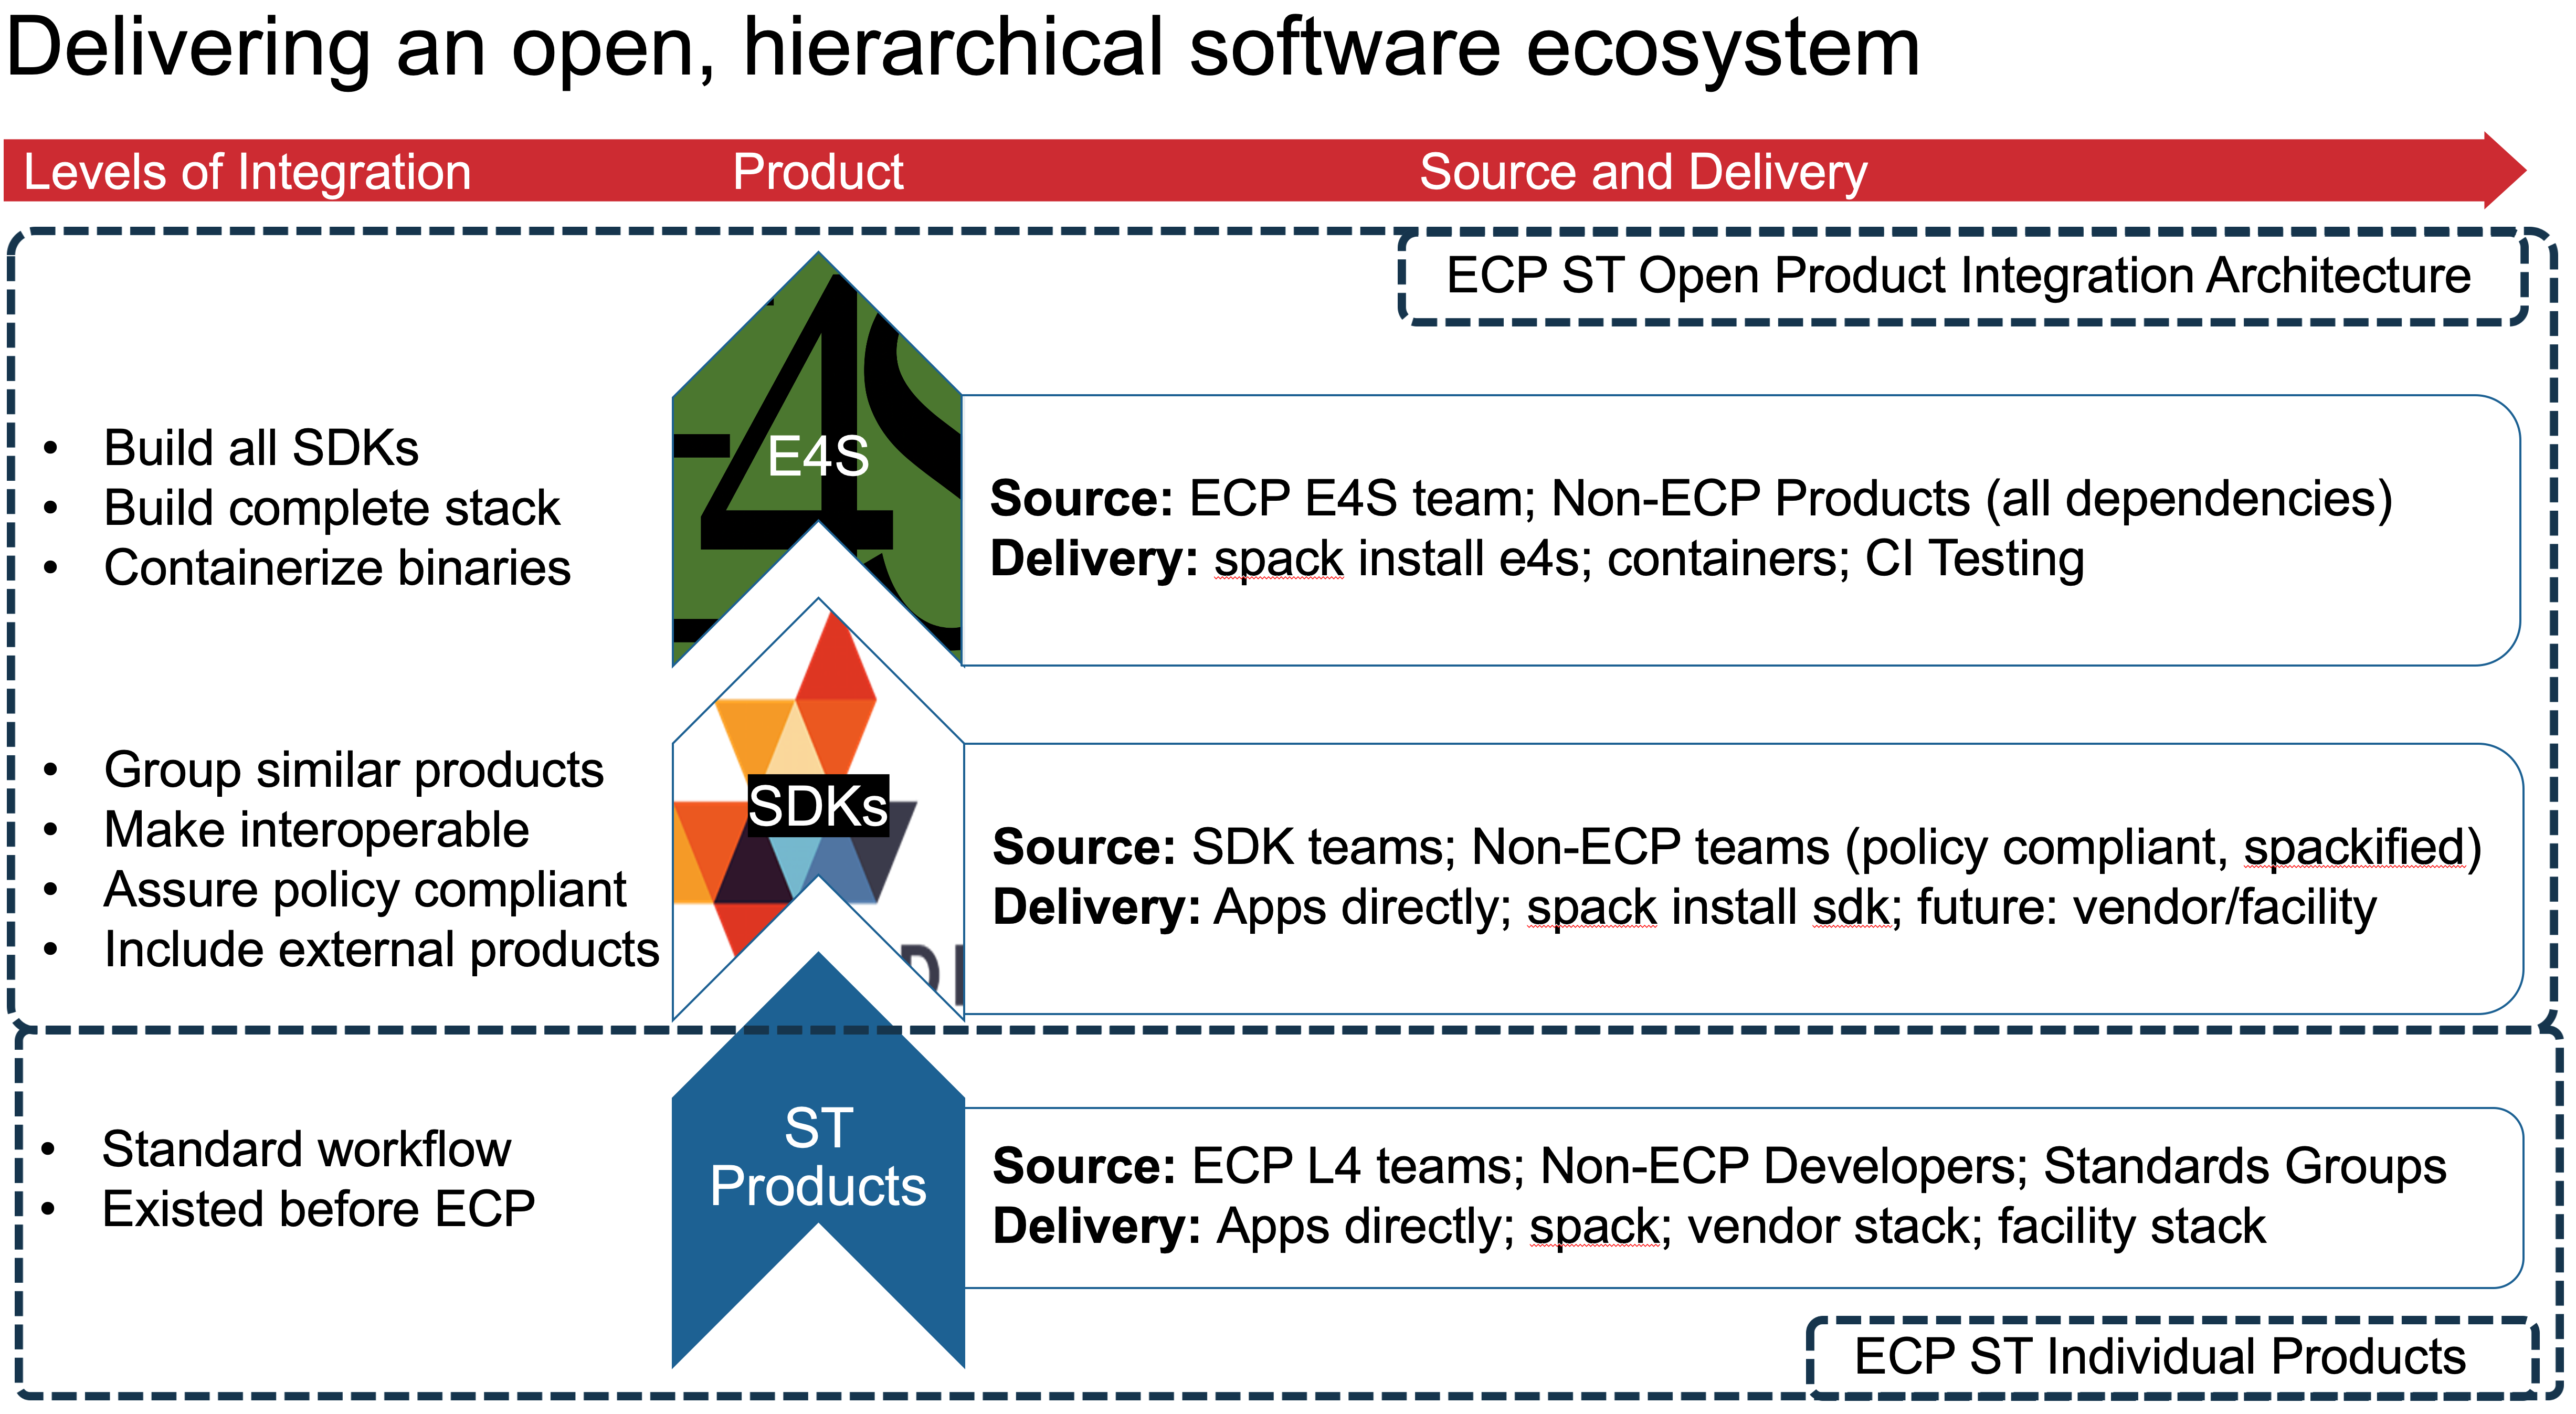
\includegraphics[width=0.9\linewidth]{E4S-Hierarchy}
	\caption{The ECP ST software stack is delivered to the user community through several channels, including via source code, using SDKs, direct to facilities in collaboration with ECP HI, and via binary distributions from containers and HPC vendors.
	Increasingly, E4S is the primary pathway for delivering ECP ST capabilities.  E4S provides testing, a documentation portal, and quality commitments via community policies.}
	\label{fig:hierarchy}
    \protect\todo[inline]{Please replace image with higher resolution image that is not a screenshot so that the image is not blurry and no longer has the red spellcheck underline.}
    \protect\todo[inline]{Capitalize: Spack, SDK, E4S, Spackified.}
\end{figure}

\subsubsection{ECP ST Software Life Cycle}
This section discusses the ECP ST software life cycle, as shown in Figure~\ref{fig:lifecycle}.  From their inception as P6 Activity planning packages, which are refined annually and given detailed information from before starting the activity all the way to the successful integration of a capability into the client environment, ECP ST features are governed by this life cycle.  Each product team conducts its own integration planning that incorporates other funding sources and stakeholders, but the ECP ST life cycle intersects the product life cycle for capabilities that the ECP funds.

\begin{figure}
	\centering
	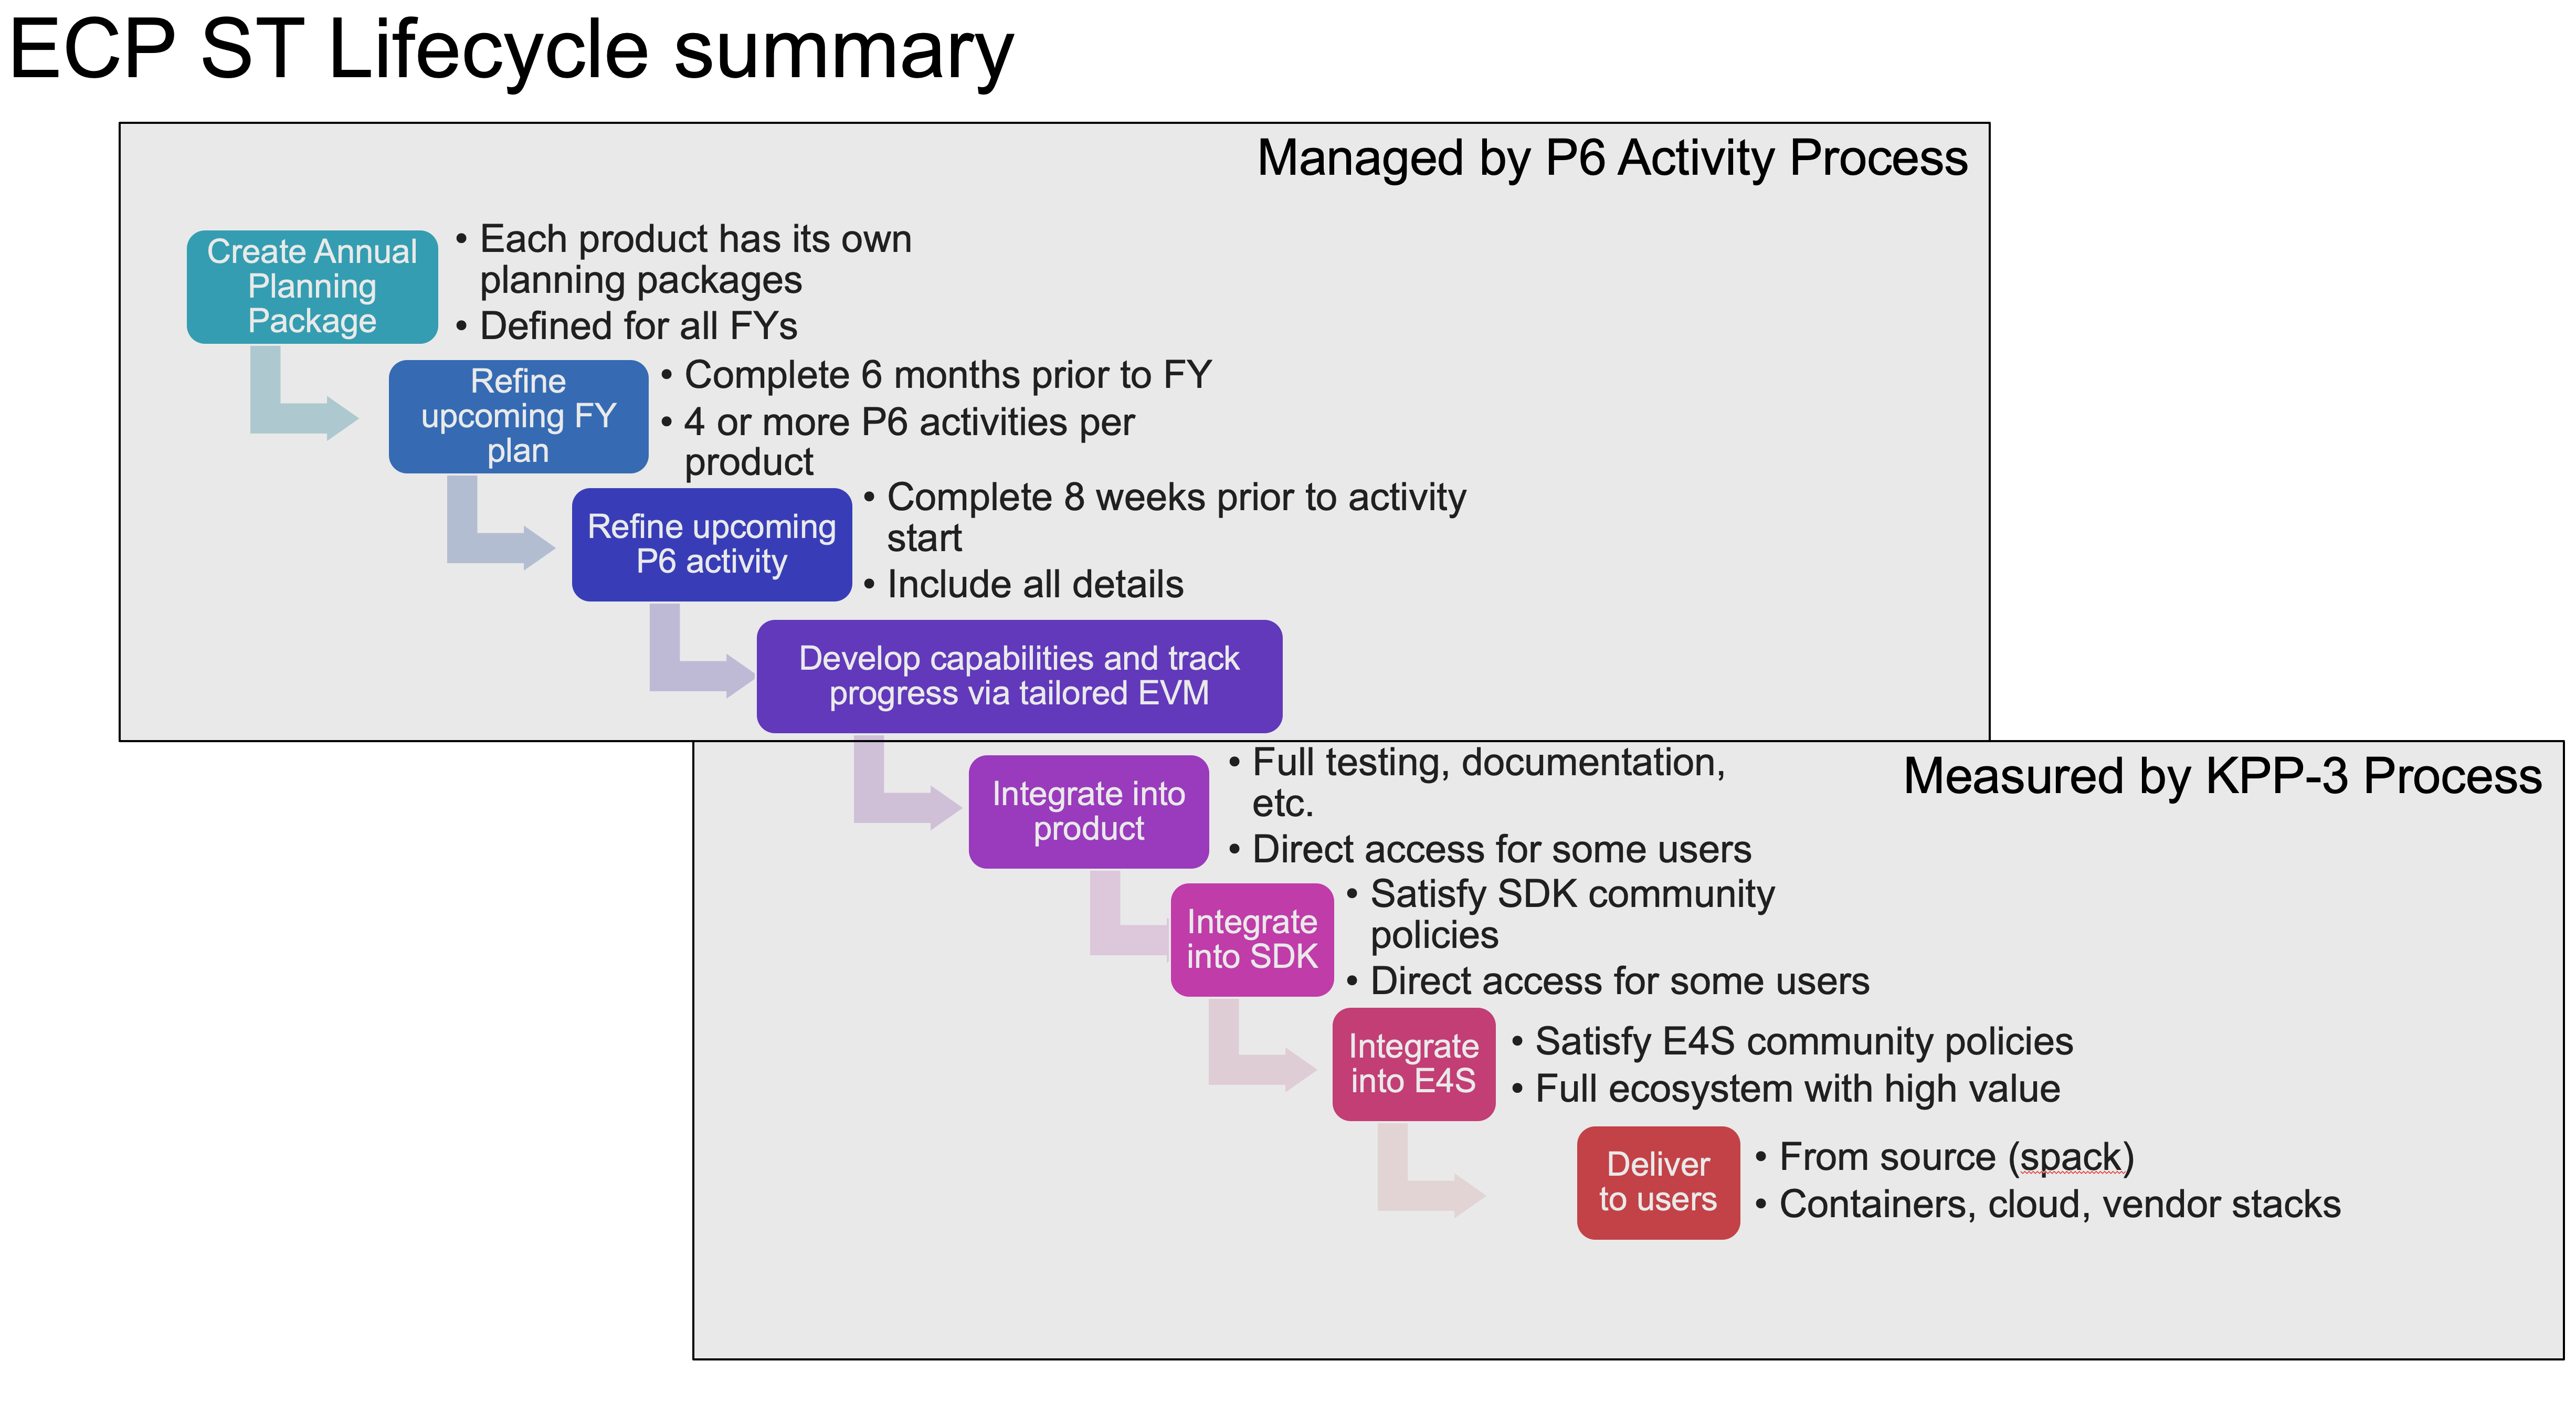
\includegraphics[width=0.9\linewidth]{E4S-Lifecycle}
	\caption{ECP ST product planning, execution, testing, and assessment are governed by the combination of P6 Activities for hierarchical planning (Figure~\ref{fig:planning-process}) and KPP-3 for measuring capability integrations (Table~\ref{table:KPP-3-scoring}).  This figure shows how the entire life cycle of ECP ST feature development is captured by these two elements.}
	\label{fig:lifecycle}
    \protect\todo[inline]{Please replace image with higher resolution image that is not a screenshot so that the image is not blurry and no longer has the red spellcheck underline. Also, if possible to edit image, please change "Lifecycle" to "Life Cycle" (it is two words per Merriam-Webster.)}
    \protect\todo[inline]{Capitalize Spack. Spell out numbers zero through nine.}
\end{figure}

